\chapter{Unraveling the sequence determinants of environment-induced changes in pancreatic $\beta$-cell states}
\label{chap:chapter 3}

%%%%%%%%%%%%%%%%%%%%%%%%%%%%%%%%%%%%%%%%%%%%%%%%%%%%%%%%%%%%%%%%%%%%%%%%%%%%%%%%
\section{Abstract}
%%%%%%%%%%%%%%%%%%%%%%%%%%%%%%%%%%%%%%%%%%%%%%%%%%%%%%%%%%%%%%%%%%%%%%%%%%%%%%%%

Environmental signals shape pancreatic $\beta$-cell function and contribute to diabetes risk. However, the mechanisms by which these signals interact with genetic variation to influence gene regulation in $\beta$-cells remains incompletely understood. Here, we present a framework for identifying sequence determinants of environment-induced gene regulatory changes in $\beta$-cell states. Using a stem cell-derived organoid model of human islets (SC-islets) exposed to four stimuli across four timepoints, we profiled over 170k nuclei for paired gene expression and chromatin accessibility, and over 14k nuclei for paired DNA methylation and chromatin organization in SC-islets. We characterized condition specific responses within each modality, identifying thousands of differentially expressed genes and accessible regions, as well as global methylation changes. We then trained sequence-to-function models to predict chromatin accessibility and CpG methylation from DNA sequence, with chromatin accessibility models capturing cell type and condition specific regulatory logic and showing strong performance in our evaluations of non-coding variant effect prediction. Our results support using multiomics in stimulated SC-islets as a framework to study context-dependent gene regulation and interpret genetic variants relevant to disease.

%%%%%%%%%%%%%%%%%%%%%%%%%%%%%%%%%%%%%%%%%%%%%%%%%%%%%%%%%%%%%%%%%%%%%%%%%%%%%%%%
\section{Introduction}
%%%%%%%%%%%%%%%%%%%%%%%%%%%%%%%%%%%%%%%%%%%%%%%%%%%%%%%%%%%%%%%%%%%%%%%%%%%%%%%%

Pancreatic islets are small clusters of endocrine cells that regulate the metabolism of glucose. Among the endocrine cell types, $\beta$-cells play a central role by producing and secreting insulin in response to intrinsic and extrinsic signals \cite{Prentki2013-vx}. While glucose is the principal stimulus for $\beta$-cell mediated insulin secretion, $\beta$-cell function is also modulated by an array of additional signals, including fatty acids \cite{Fu2013-cf,Mauvais-Jarvis2016-gm,Ramos-Rodriguez2019-ha,Aylward2021-nw}, amino acids \cite{Newsholme2007-xy}, incretin hormones \cite{Saxena2010-ui}, proinflammatory cytokines \cite{Benaglio2022-rq}, glucocorticoids \cite{Aylward2021-nw,Reddy2009-qu}, and sex hormones \cite{Mauvais-Jarvis2016-gm}. A subset of these molecules have been shown to alter the broader transcriptional and epigenomic landscape of $\beta$-cells \cite{Aylward2021-nw,Benaglio2022-rq,Ramos-Rodriguez2019-ha}, revealing widespread, time-dependent changes in histone modifications, chromatin accessibility, and gene expression \cite{Ramos-Rodriguez2019-ha,Benaglio2022-rq}. 

These responses primarily reflect modulation of pre-existing cis-regulatory elements (CREs), which are frequently enriched for both transcription factor (TF) binding motifs relevant to the applied stimulus and glucose-associated genetic variants identified through genome-wide association studies (GWAS). GWAS variants for fasting glucose \cite{Ingelsson2010-tw,Manning2012-ro,Scott2012-hq,Wood2017-uc,Williamson2023-gf} and type 2 diabetes (T2D) \cite{Mahajan2022-hu} are strongly enriched in CREs active in pancreatic islets \cite{Liu2016-on,Pasquali2014-cu}. Within islets, this enrichment is pronounced in regulatory regions specific to $\beta$-cells \cite{Chiou2021-ro}. For instance, variants near MTNR1B, a locus contributing substantially to fasting glucose heritability, have been shown to alter $\beta$-cell enhancer activity \cite{Prokopenko2009-ou}. More comprehensively elucidating the mechanisms by which non-coding variants impact beta-cell regulatory programs remains a major challenge, particularly when a certain environmental context is necessary for the effect to be observed.

%GWAS variants for fasting glucose \cite{Ingelsson2010-tw,Manning2012-ro,Scott2012-hq,Wood2017-uc,Williamson2023-gf} and type 2 diabetes \cite{Dupuis2010-ws,Morris2012-uu,Mahajan2022-hu} are strongly enriched in CREs active in pancreatic islets \cite{Liu2016-on,Pasquali2014-cu}. Within islets, this enrichment is pronounced in regulatory regions specific to $\beta$-cells \cite{Chiou2021-ro}. For instance, variants near MTNR1B, a locus contributing substantially to fasting glucose heritability, have been shown to alter $\beta$-cell enhancer activity \cite{Prokopenko2009-ou}. More comprehensively elucidating the mechanisms by which non-coding variants impact beta-cell regulatory programs remains a major challenge, particularly when a certain environmental context is necessary for the effect to be observed.

Given the central role of islets in diabetes pathogenesis, the islet epigenome has been the focus of extensive investigation \cite{Pasquali2014-cu,Gaulton2010-mq,Greenwald2019-ou,Khetan2018-fm,Thurner2018-ln,Volkov2017-tz}. Most of these data have been derived from bulk islet tissue, limiting the ability to resolve contributions from individual cell types. Recent advances in single-cell technologies have enabled high-resolution epigenomic profiling at the level of individual cells. Including multimodal platforms that simultaneously measure combinations of chromatin accessibility, gene expression, DNA methylation, and three-dimensional genome architecture \cite{Lee2019-qo,Liu2021-km}. Our group and others have recently generated single-cell chromatin accessibility maps from healthy human islets, revealing regulatory elements active in $\beta$-cells and uncovering previously unappreciated heterogeneity within the $\beta$-cell population \cite{Chiou2021-ro,Rai2020-cf,Wang2023-me}.

Primary human islets, however, are currently not amenable to genetic manipulation, which limits their utility for validating the functional consequences of variants. Transformed human $\beta$-cell lines \cite{Ravassard2011-lj} offer an alternative but face significant limitations, including the absence of interactions with other endocrine cell types \cite{Rutter2013-yv}. Human pluripotent stem cell (hPSC)-derived islet organoids (SC-islets) help overcome these barriers by recapitulating the major endocrine populations present in native islets \cite{Hogrebe2020-rr,Rezania2014-nz,Veres2019-qb,Velazco-Cruz2019-yq,Zhu2023-qm} while providing a genetically tractable system for targeted genome editing \cite{Komor2016-px}. CRISPR-based perturbations in hPSC-islet organoids have enabled both fine-scale dissection of individual regulatory elements and scalable functional screening.

Deep learning models trained directly on genomic sequence have shown strong performance in predicting a range of regulatory phenotypes \cite{Sasse2024-ly}. These models learn sequence features, including combinatorial TF binding site logic, that are predictive of chromatin accessibility \cite{Pampari2025-lm}, gene expression\cite{Linder2025-or}, DNA methylation\cite{Zeng2017-kb}, and three-dimensional chromatin conformation \cite{Fudenberg2020-gs}. Because they operate on sequence alone, these models provide a natural framework for evaluating functional consequences of non-coding variants by comparing predicted outputs for reference and alternate alleles. Recently, they have successfully been applied to aid fine-mapping of variants in Type 2 diabetes \cite{Hudaiberdiev2023-ew}. As such, they represent a valuable tool for decoding the regulatory genome and prioritizing candidate variants associated with disease-relevant traits. 

%%%%%%%%%%%%%%%%%%%%%%%%%%%%%%%%%%%%%%%%%%%%%%%%%%%%%%%%%%%%%%%%%%%%%%%%%%%%%%%%
\section{Results}
%%%%%%%%%%%%%%%%%%%%%%%%%%%%%%%%%%%%%%%%%%%%%%%%%%%%%%%%%%%%%%%%%%%%%%%%%%%%%%%%

\subsection{Multiomic profiling of stem cell-derived pancreatic organoids}

To investigate the temporal response of $\beta$-cells to environmental signals, we first differentiated H1 human pluripotent stem cells (hESCs) through a stepwise protocol into SC-islets (\textbf{Figure~\ref{fig:3 Figure 1}\textbf{a}}) \cite{Hogrebe2020-rr,Rezania2014-nz,Veres2019-qb,Velazco-Cruz2019-yq,Zhu2023-qm}. Following differentiation, we introduced four different stimuli to the cell culture media: 1) a cocktail of three cytokines (3-cyt), 2) IFN$\gamma$ alone (IFN$\gamma$), 3) Exendin-4 in the presence of high glucose (Exendin-4), and 4) palmitate. We collected aliquots of each treated culture at four timepoints (6, 24, 48, and 72 hours), alongside a control time course of unstimulated organoids with an additional baseline timepoint (0 hr). We then performed multiomic single-cell profiling across conditions and timepoints using two assays in replicate. Using the 10x Genomics Multiome platform, we simultaneously measured chromatin accessibility and gene expression from the same nuclei, and using snm3C-seq we jointly profiled DNA methylation and 3D chromatin architecture \cite{Liu2021-km}. Each sample was subjected to systematic quality control to filter out low quality nuclei (\textbf{Supplementary Figure~\ref{fig:3 supplementary_1}}, \textbf{Supplementary Table 1}, see Methods). In total, we profiled 171{,}815 nuclei using 10x Multiome and 14{,}197 nuclei using snm3C-seq.

We performed unsupervised clustering on gene expression (10x Multiome) and DNA methylation (snm3C-seq) profiles to identify major islet endocrine cell types (\textbf{Figure~\ref{fig:3 Figure 1}\textbf{c}}, \textbf{Supplementary Figure~\ref{fig:3 supplementary_1}\textbf{a}}). Cell type labels were assigned based on known marker genes (\textbf{Supplementary Figure~\ref{fig:3 supplementary_1}\textbf{b}}), with clusters corresponding to SC-alpha cells (purple), SC-beta (blue), SC-EC (orange), and SC-delta (red) cells. While SC-delta cells were readily identifiable in the RNA space via \textit{SST} expression, they did not form distinct clusters in the DNA methylation space, likely reflecting their low abundance or less distinctive methylation profile in this context. We examined cell type proportions across stimuli and timepoints for each assay (\textbf{Figure~\ref{fig:3 Figure 1}\textbf{e}}). Despite differences in the number of cells captured per condition, the relative distribution of SC-alpha, SC-beta, and SC-EC cells remained broadly consistent across assays and conditions. To facilitate downstream comparisons between molecular modalities, we aggregated sequencing reads within each cell type to construct cell type resolved transcriptome and epigenome maps at multiple resolutions, including across all measured conditions (\textbf{Figure~\ref{fig:3 Figure 1}\textbf{h}}). At a sample level, pseudobulked modalities exhibited strong correlations across genes in the expected directions (\textbf{Supplementary Figure~\ref{fig:3 supplementary_2}\textbf{c}}).

\clearpage
\thispagestyle{plain}
\noindent
\textbf{Figure~\ref{fig:3 Figure 1}. Multiomic profiling of hESC-derived islet organoids across environmental conditions}. \textbf{a}, Schematic of directed differentiation from H1 hESCs into islet organoids followed by stimulation with one of four environmental conditions across four timepoints. Multiomic single-cell assays were used to capture single-cell mRNA, chromatin accessibility, DNA methylation and chromatin conformation profiles. \textbf{b}, UMAP embeddings for cells across all conditions with cell type labels, divided into mRNA expression (RNA), chromatin accessibility (ATAC), DNA methylation (mCG), and 3D chromatin contacts (3C) . \textbf{c}, Bar plots showing the number and relative proportion of cells per cell type across conditions and timepoints for 10x Multiome and snm3C-seq. \textbf{d}, Representative genome browser tracks at the INS locus (and downstream) showing chromatin accessibility, DNA methylation, mRNA expression and HiC profiles for SC-alpha, SC-beta, and SC-EC cells aggregated across all conditions.

\clearpage

\begin{figure}[!htbp]
    \centering
    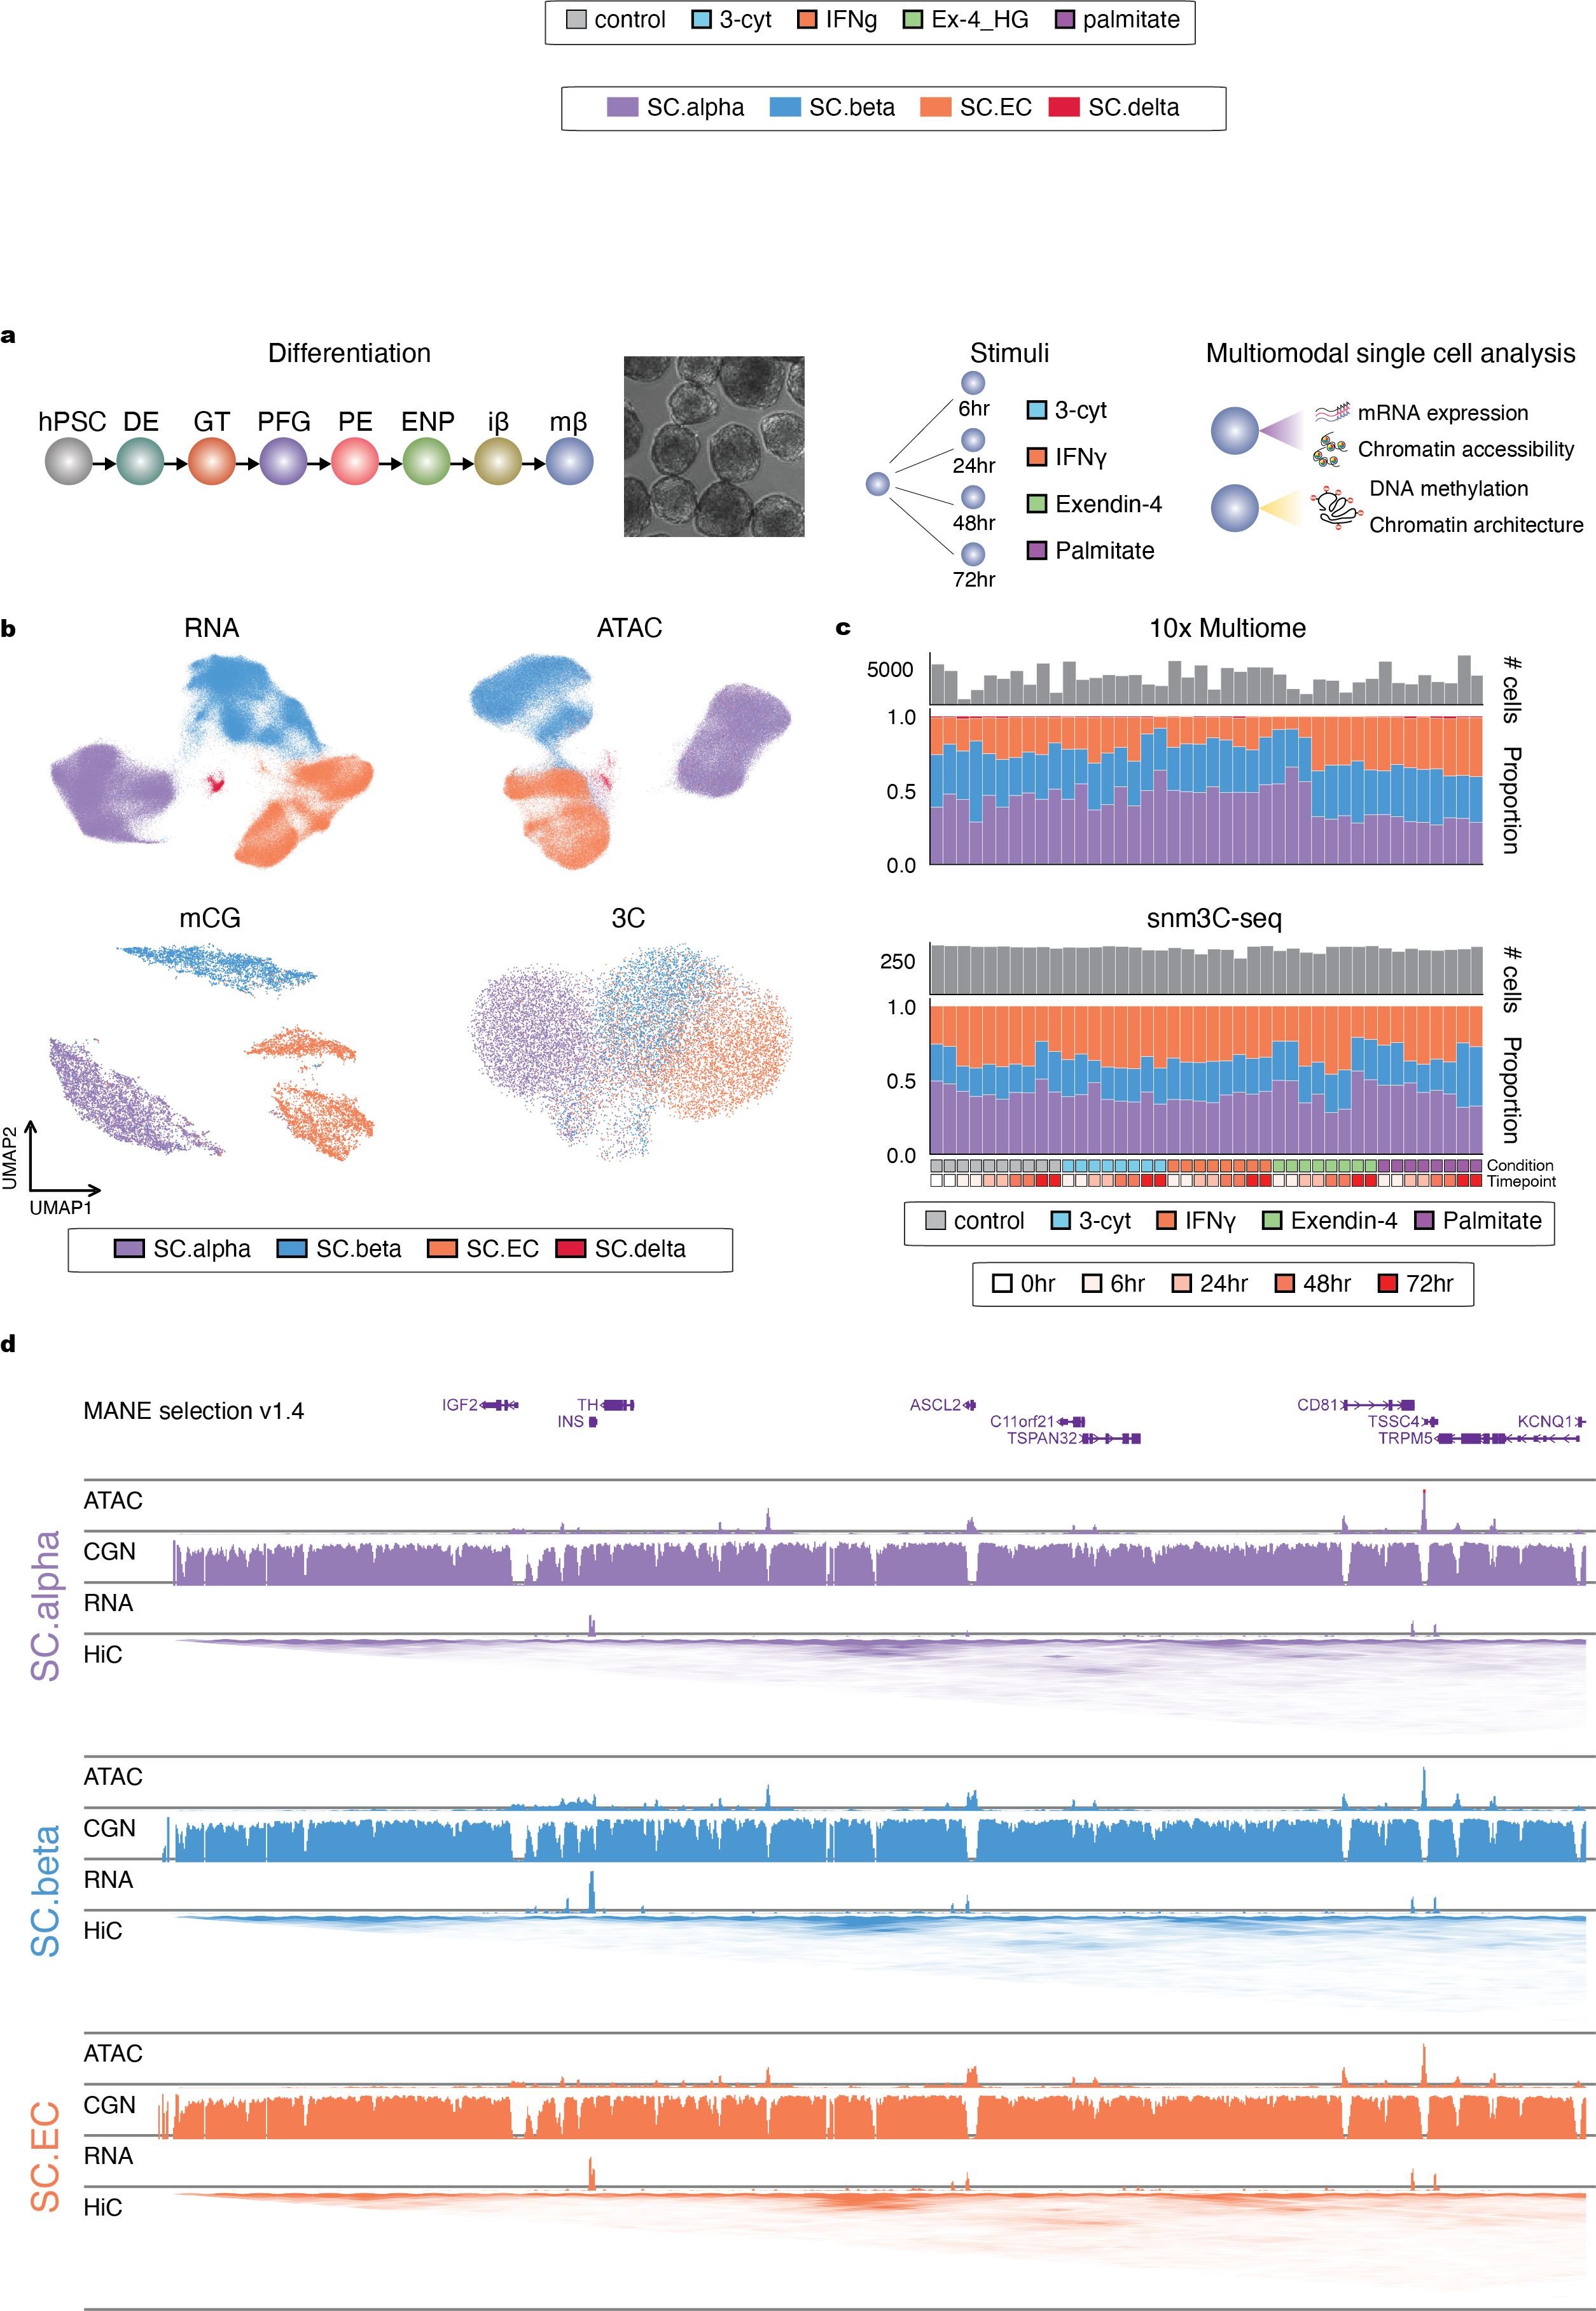
\includegraphics[height=0.8\textheight, keepaspectratio]{3_figures-and-files/Fig1.png}
    \caption[Multiomic profiling of hESC-derived islet organoids]{\textbf{Multiomic profiling of hESC-derived islet organoids}.}
    \label{fig:3 Figure 1}
\end{figure}

\clearpage

%%%%%%%%%%%%%%%%%%%%%%%%%%%%%%%%%%%%%%%%%%%%%%%%%%%%%%%%%%%%%%%%%%%%%%%%%%%%%%%%

\subsection{Treatments induce variable transcriptomic response in SC-beta cells}

To assess how each stimulus affected gene expression in SC-beta cells, we first generated pseudobulk transcriptomes by aggregating snRNA-seq counts across SC-beta labeled cells from each sample. We then performed differential gene expression analysis using DESeq2 to identify genes with condition specific changes at any point across the time course (see Methods). We observed the strongest transcriptomic responses in SC-beta cells exposed to proinflammatory cytokines (\textbf{Figure~\ref{fig:3 Figure 2}\textbf{a}}), with 3-cyt and IFN$\gamma$ inducing 615 and 2,781 differentially expressed genes (DEGs) respectively at an FDR of 5\% (\textbf{Figure~\ref{fig:3 Figure 2}\textbf{b}}). In contrast, Exendin-4 and palmitate induced subtler changes (\textbf{Figure~\ref{fig:3 Figure 2}\textbf{b}}), with 126 and 46 DEGs respectively at an FDR of 25\%. Notably, several of the genes induced by Exendin-4, including \textit{SLC8A1} \cite{Hamming2010-td}, \textit{PDK4} \cite{Arumugam2010-bq}, and \textit{TXNIP}, are known components of the $\beta$-cell response to glucose stimulation. \textit{TXNIP}, in particular, has been reported to be strongly upregulated in diabetic islets and is linked to $\beta$-cell stress responses \cite{Rutter2013-yv}. A significant proportion of DEGs were shared among 3-cyt and IFN$\gamma$ responses and the Exendin-4 and IFN$\gamma$, but we observed minimal overlap among other conditions (\textbf{Supplementary Figure~\ref{fig:3 supplementary_3}\textbf{a}}).

Using decoupleR \cite{Badia-I-Mompel2022-se}, we inferred TF activities across conditions (\textbf{Supplementary Figure~\ref{fig:3 supplementary_3}\textbf{b}}). The cytokine treatments (3-cyt, IFN$\gamma$) prominently activated downstream targets of known immune regulators of $\beta$-cells including STAT1, IRF1, and CIITA \cite{Benaglio2022-rq}. As expected, NF-$\kappa$B was upregulated in 3-cyt and not IFN$\gamma$ \cite{Melloul2008-ox}. Under palmitate treatment, we observed reduced activity of HNF1B and ISL1, both of which are essential for maintaining mature $\beta$-cell identity \cite{El-Khairi2016-so,Ediger2014-gk}. TFEB, a regulator of lysosomal biogenesis and autophagy, was strongly upregulated in response to Exendin-4, consistent with reports that GLP-1 agonists activate TFEB via calcium/calcineurin signaling to enhance autophagic flux and improve $\beta$-cell survival \cite{Zummo2022-dr}. In contrast, TFEB activity was consistently suppressed in response to both palmitate and cytokines. Exendin-4 also led to downregulation of several GATA6 targets, consistent with studies showing that GATA6 knockdown impairs $\beta$-cell function and identity \cite{Villamayor2018-uk}. PIAS1 was one of the few transcriptional regulators significantly upregulated under Exendin-4 treatment. As an E3 SUMO ligase, PIAS1 modulates post-translational SUMOylation of TFs, a pathway previously implicated in $\beta$-cell stress adaptation and survival \cite{Li2020-kg}.

To further resolve shared and condition specific transcriptional responses, we performed unsupervised clustering of differentially expressed genes across all conditions, identifying 43 gene clusters (\textbf{Figure~\ref{fig:3 Figure 2}\textbf{c}}). Gene ontology enrichment analysis revealed that these clusters capture a range of functional annotations (\textbf{Figure~\ref{fig:3 Figure 2}\textbf{d}}). For example, Cluster 16 genes exhibited an immediate and sustained upregulation in response to cytokine treatments and were strongly enriched for terms related to interferon signaling. Cluster 4 genes were induced at later timepoints in the palmitate and control conditions and were enriched for synaptic signaling and glutamate receptor activity. Cluster 6 genes were also marked by a delayed upregulation, most pronounced under palmitate exposure, and included genes involved in fructose metabolism and AMPK signaling. Cluster 58 genes included those involved in structural remodeling programs, with enrichment for collagen organization and hydroxylation pathways that increased at later timepoints in palmitate and control. As a final example, Cluster 35 captured canonical inflammatory stress responses to TNF$\alpha$ signaling and was sharply induced by only the 3-cytokine cocktail. These clusters highlight the range of early and delayed gene programs engaged across stimuli, spanning immune activation, metabolic compensation, and cell structure remodeling.

\clearpage

\thispagestyle{plain}
\noindent
\textbf{Figure~\ref{fig:3 Figure 2}. Transcriptomic responses of SC-beta cells to environmental stimuli}. \textbf{a}, Principal component analysis of pseudobulked SC-beta cell transcriptomes across all conditions and timepoints. Each point represents a sample, colored by treatment. \textbf{b}, Volcano plots showing differentially expressed genes in SC-beta cells at any timepoint relative to control for each stimulus. From top left to bottom right: 3-cyt, IFN$\gamma$, exendin-4, and palmitate. Red points denote genes with $\log\mathrm{FC} > 0.5$ and FDR $< 0.05$ for cytokines or FDR $< 0.25$ for exendin-4 and palmitate. Blue points denote genes with $\log\mathrm{FC} < -0.5$ and FDR below the same respective thresholds. Numbers indicate up- and down-regulated genes. \textbf{c}, Heatmap of $Z$-scored gene expression across timepoints for each treatment in SC-beta cells. DEGs are grouped into clusters based on temporal expression dynamics. \textbf{d}, Representative expression profiles for five selected gene clusters across the time course. Right panels show GO term enrichments associated with each cluster (top five terms shown, ordered by adjusted $p$-value).

\clearpage

\begin{figure}[!htbp]
    \centering
    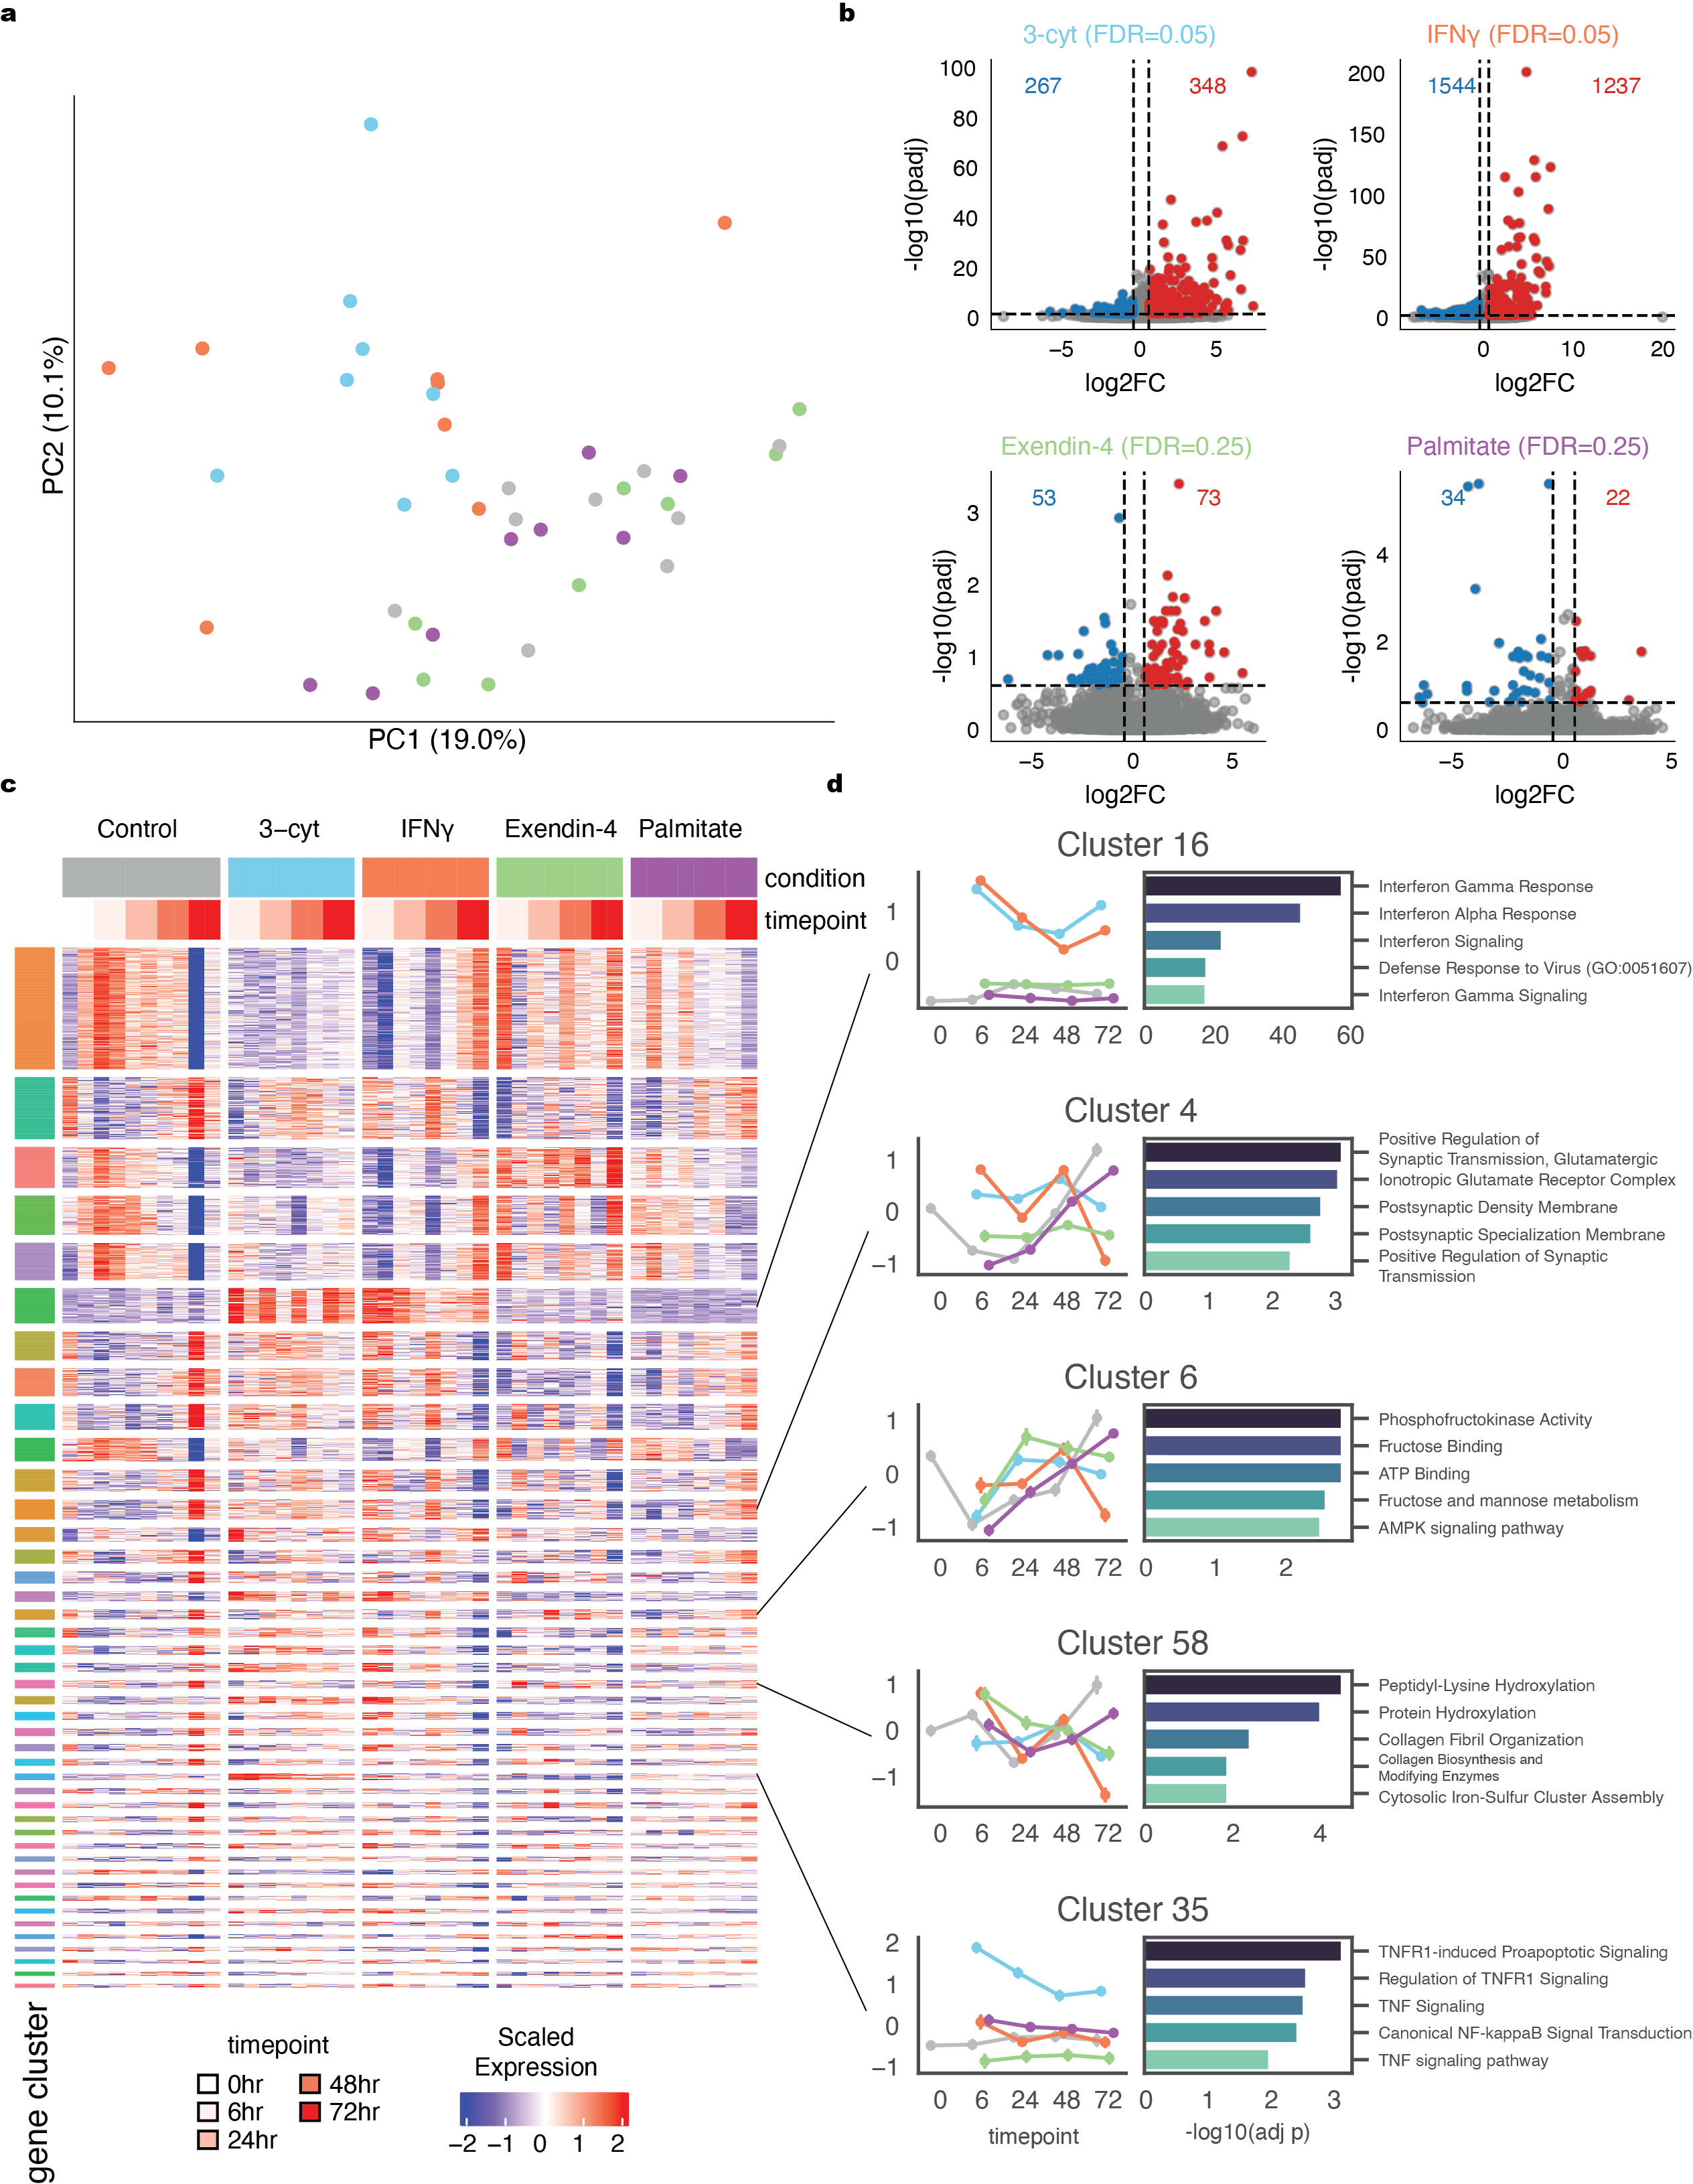
\includegraphics[height=0.8\textheight, keepaspectratio]{3_figures-and-files/Fig2.png}
    \caption[Transcriptomic responses of SC-beta cells to environmental stimuli]{\textbf{Transcriptomic responses of SC-beta cells to environmental stimuli}.}
    \label{fig:3 Figure 2}
\end{figure}

\clearpage

%%%%%%%%%%%%%%%%%%%%%%%%%%%%%%%%%%%%%%%%%%%%%%%%%%%%%%%%%%%%%%%%%%%%%%%%%%%%%%%%

\subsection{Cytokines induce strong changes in chromatin accessibility}

We next performed a parallel analysis to evaluate how environmental stimuli influence chromatin accessibility in SC-beta cells. As with the transcriptome analysis, we aggregated counts across samples, this time using raw Tn5 insertion counts in consensus peaks (see Methods). We then performed differential accessibility analysis for each condition relative to baseline using DESeq2. The largest changes in SC-beta chromatin accessibility were again observed in response to cytokine exposure (\textbf{Figure~\ref{fig:3 Figure 3}\textbf{a}}). Treatment with 3-cyt and IFN$\gamma$ led to 1,148 or 1,536 differentially accessible peaks, respectively (\textbf{Figure~\ref{fig:3 Figure 3}\textbf{b}}). Almost all peaks increased in accessibility, with a large proportion of upregulated differentially accessible regions (DARs) shared between the cytokine treatments (\textbf{Supplementary Figure~\ref{fig:3 supplementary_3}\textbf{c}}). In contrast, Exendin-4 and palmitate induced negligible chromatin changes, even at a relaxed FDR threshold of 25\% (\textbf{Figure~\ref{fig:3 Figure 3}\textbf{b}}). We observed subtle but significant differences in peak annotation and distance from the TSS (\textbf{Supplementary Figure~\ref{fig:3 supplementary_3}\textbf{d}}) between DARs and stable peaks. Overall, these results suggest that cytokines drive coordinated changes in both gene expression and CRE activity in SC-beta cells.

We next clustered differentially accessible peaks across the time course, identifying 46 distinct patterns of accessibility dynamics (\textbf{Figure~\ref{fig:3 Figure 3}\textbf{c}}). HOMER \cite{Heinz2010-yo} TF motif enrichment analysis uncovered clear regulatory signatures across clusters. Cytokine treatments produced the most pronounced chromatin changes, with multiple clusters showing sharp changes in accessibility. For example, Cluster 7 peaks showed strong induction in both the 3-cyt and IFN$\gamma$ conditions and were enriched for IRF and STAT motifs, consistent with interferon signaling. Cluster 5 peaks showed a rapid but IFN$\gamma$-specific decrease in accessibility, and were enriched for NF-$\kappa$B motifs. In contrast, palmitate induced more modest chromatin changes, but several peak clusters showed delayed stimulation unique to this condition. Cluster 9 and Cluster 23 peaks, for instance, exhibited a gradual increase in accessibility under palmitate and were enriched for FOX family motifs and an NKX6-1 motif respectively, both key regulators of $\beta$-cell identity and function \cite{Geusz2021-mr,Lantz2004-mi,Aigha2020-uu}. Cluster 22, on the other hand, exhibited a gradual decrease in accessibility in palmitate treated SC-beta cells and was enriched for RFX motifs \cite{Piccand2014-bd}. This suggests that palmitate gradually activates regulatory elements linked to FOXA and NKX6-1, while repressing RFX-associated regions over time, a shift that may mark a transition from compensatory to dysfunctional $\beta$-cell states.

\clearpage

\thispagestyle{plain}
\noindent
\textbf{Figure~\ref{fig:3 Figure 3}. Chromatin accessibility dynamics in SC-beta cells in response to environmental stimuli}. \textbf{a}, Principal component analysis of pseudobulk chromatin accessibility profiles from SC-beta cells across all conditions and timepoints. \textbf{b}, Volcano plots showing differentially accessible peaks in SC-beta cells at any timepoint relative to baseline for each stimulus. From top left to bottom right: 3-cyt, IFNg, exendin-4, and palmitate. Red points denote peaks with log2FC > 0.5 and FDR < threshold (0.05 for cytokines, 0.25 for exendin-4, and palmitate). Blue points denote peaks with log2FC < 0.5 and FDR < threshold. Numbers indicate up- and down-regulated genes. \textbf{c}, Heatmap showing Z-scored accessibility for dynamic peaks across timepoints and conditions in SC-beta cells. DARs are grouped into clusters based on temporal accessibility profiles. \textbf{d}, Representative accessibility profiles for five selected clusters, with HOMER motif enrichment results shown on the right. Top five enriched motifs per cluster are listed and ranked by adjusted p-value.

\clearpage

\begin{figure}[!htbp]
    \centering
    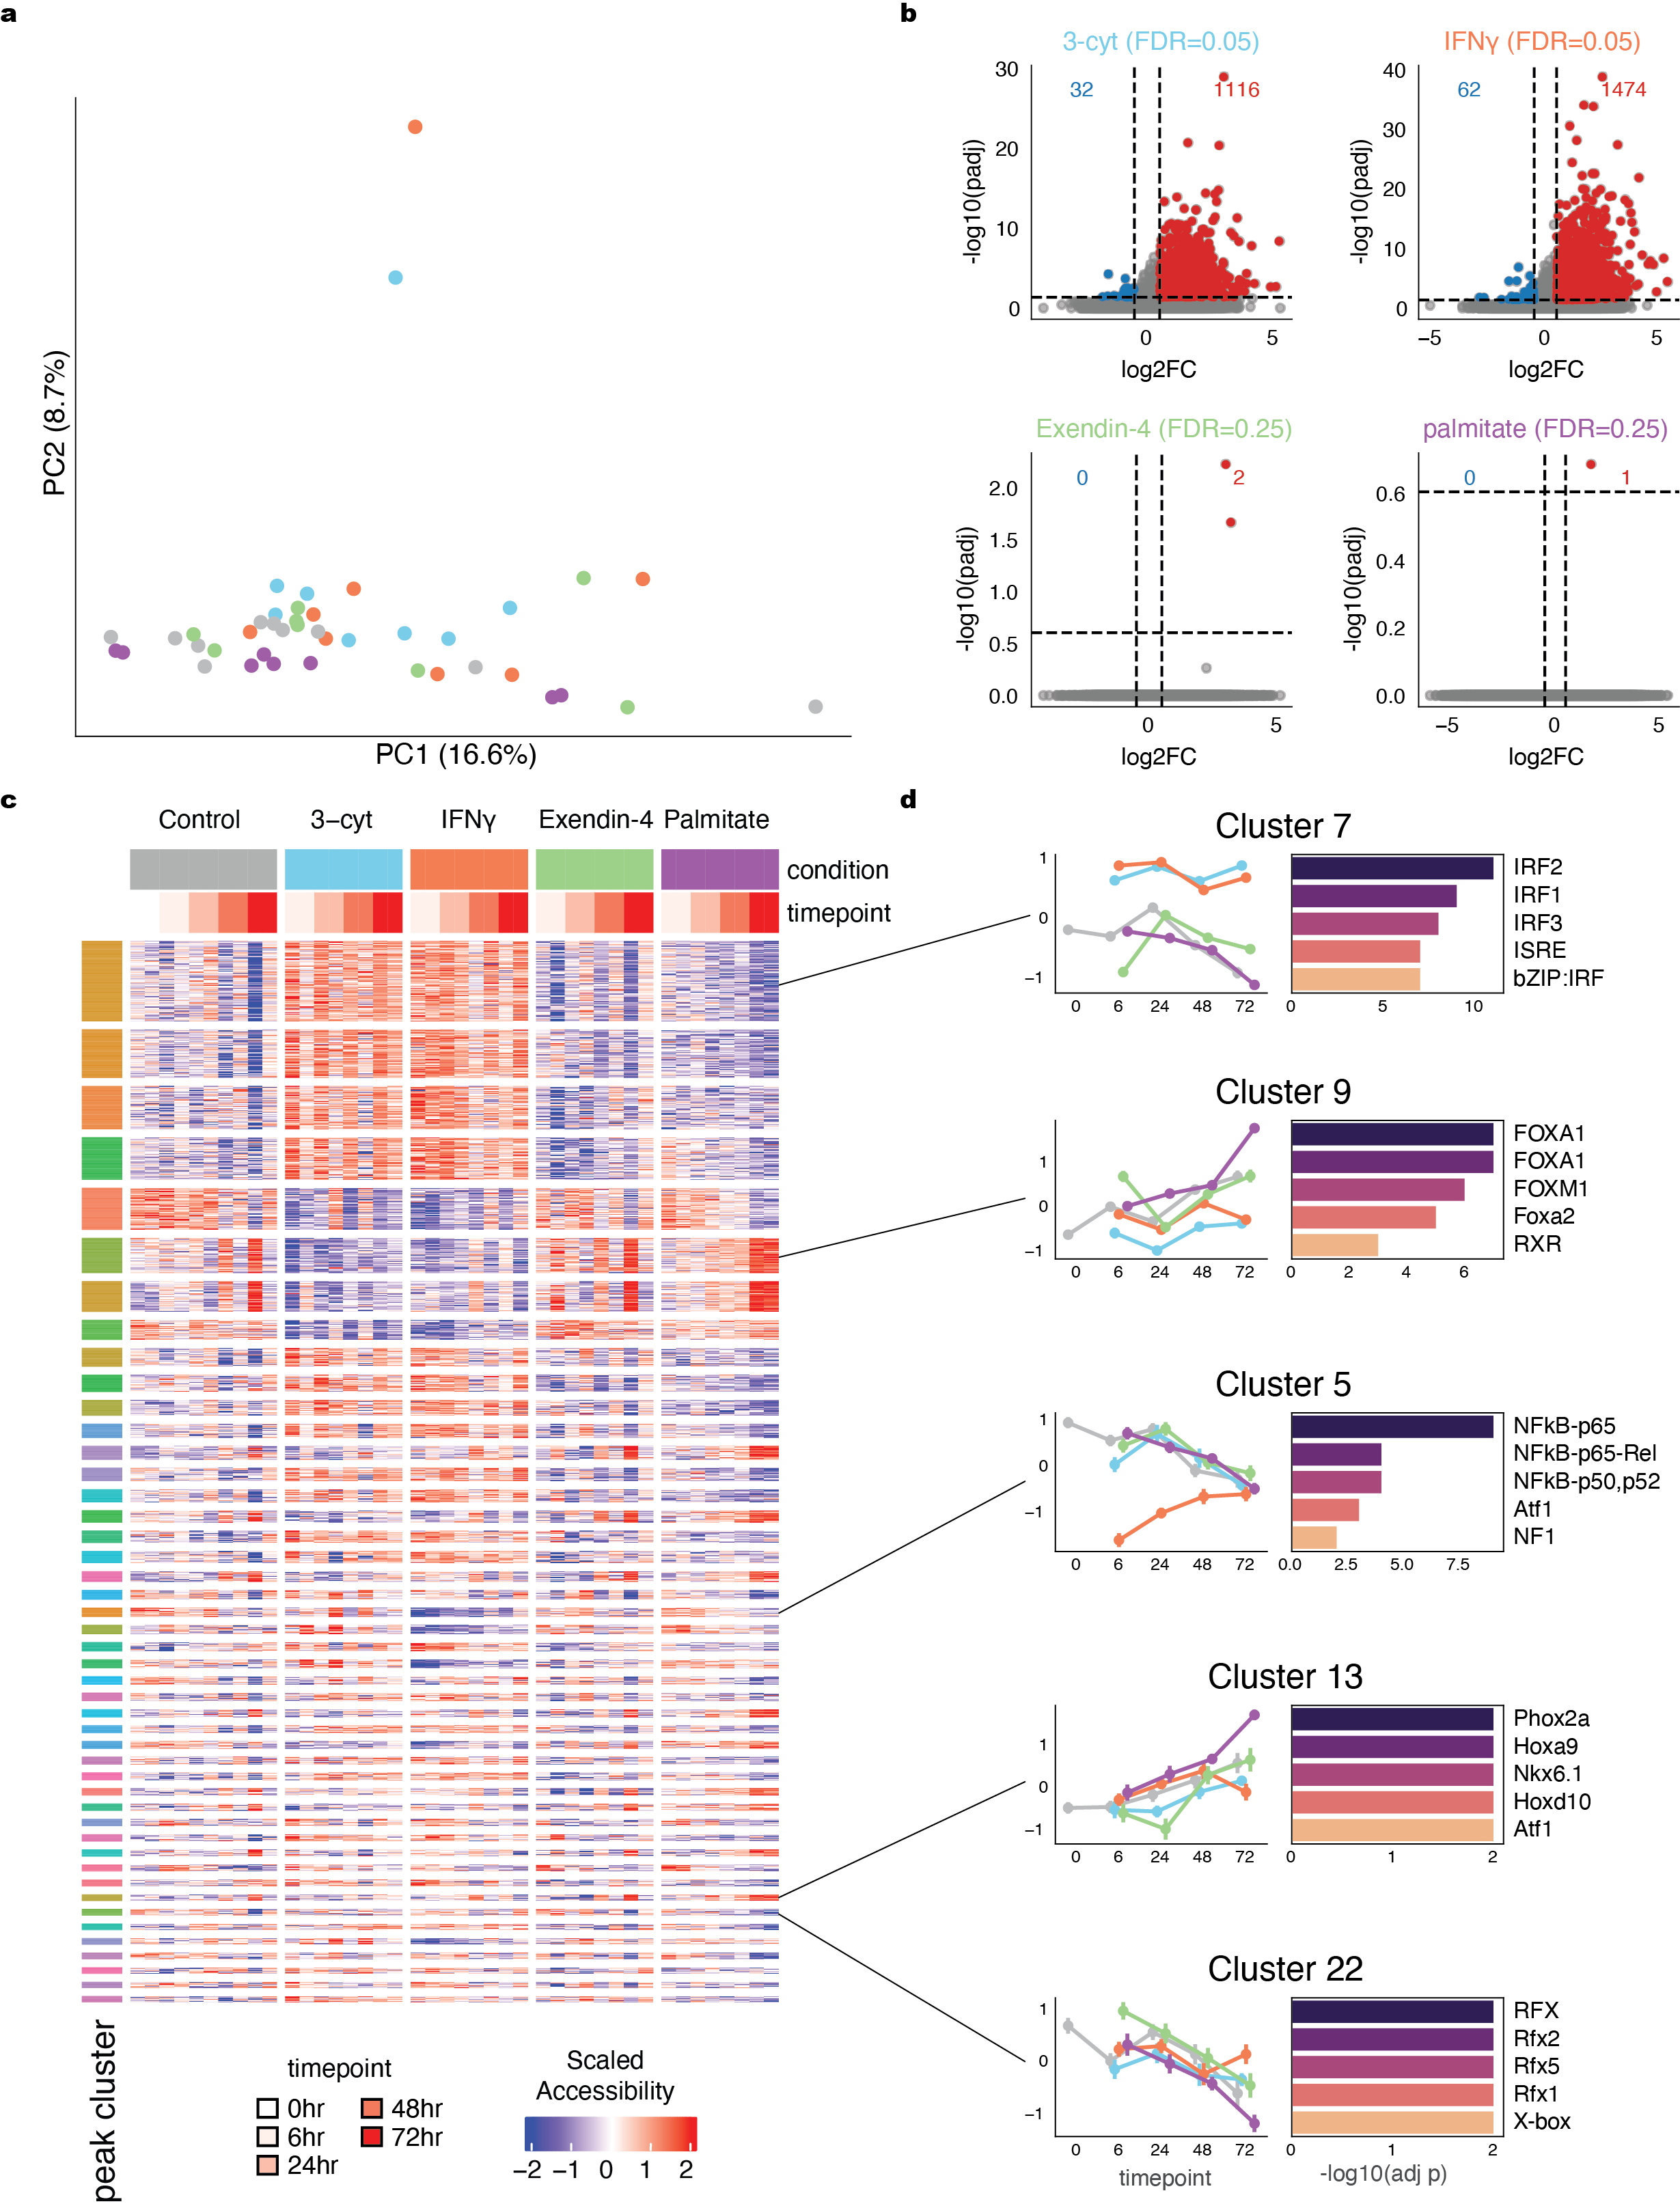
\includegraphics[height=0.8\textheight, keepaspectratio]{3_figures-and-files/Fig3.png}
    \caption[Chromatin accessibility dynamics in SC-beta cells in response to environmental stimuli]{\textbf{Chromatin accessibility dynamics in SC-beta cells in response to environmental stimuli}.}
    \label{fig:3 Figure 3}
\end{figure}

\clearpage

%%%%%%%%%%%%%%%%%%%%%%%%%%%%%%%%%%%%%%%%%%%%%%%%%%%%%%%%%%%%%%%%%%%%%%%%%%%%%%%%

\subsection{Sequence-to-function neural networks capture chromatin accessibility and predict variant effects}

To uncover the sequence features driving condition specific chromatin accessibility in SC-islet organoids, we trained a series of ChromBPNet models on pseudobulked ATAC-seq fragments from each cell type and condition \cite{Pampari2025-lm}. All trained models showed strong performance, with Pearson correlation coefficients (PCCs) exceeding 0.8 for total accessibility count predictions (\textbf{Figure~\ref{fig:3 Figure 4}\textbf{a}}) and median Jensen–Shannon divergence (JSD) well below shuffled profiles (\textbf{Figure~\ref{fig:3 Figure 4}\textbf{a}}). Models were capable of capturing differential accessibility across conditions, including those observed under inflammatory stress (\textbf{Figure~\ref{fig:3 Figure 4}\textbf{b}}).

To identify learned sequence motifs that influence accessibility, we applied TF-MoDISco to base-pair contribution scores from each model \cite{Shrikumar2018-sb}. We then calculated an effect size for each motif and model combination by marginalizing the motif effect across a set of 100 background sequences (see Methods). Using an ANOVA to identify motifs that were condition and cell type specific, we found 7 motifs with condition specificity and 19 motifs with cell type specificity (\textbf{Figure~\ref{fig:3 Figure 4}\textbf{c}}). Condition-specific motifs included the canonical IRF1 dimer \cite{Kirchhoff1998-xj}, which showed a large effect across cell types for 3-cyt and IFN$\gamma$ models. We also identified several cell type specific motifs, including PAX6 (SC-beta), HNF4A (SC-alpha), and ETV6 (SC-EC). Certain motifs showed both cell type and condition specific effects, including NFKB1, which was active only in SC-alpha cells treated with 3-cyt. 

We next tested whether the models could accurately predict functional consequences of non-coding genetic variants in four ways. First, we asked whether models could prioritize fine-mapped (T2D) variants \cite{Mahajan2022-hu} against a background set (see Methods). We found that model-derived variant scores were significantly enriched for high posterior inclusion probability (PIP) SNPs, particularly in SC-beta cell models (\textbf{Figure~\ref{fig:3 Figure 4}\textbf{d}}). Second, we asked whether predictions from the SC-beta control model were concordant with caQTLs in primary human islets \cite{Mummey2024-kx}. The model captured the direction of effect but mostly underestimated effect magnitude (\textbf{Figure~\ref{fig:3 Figure 4}\textbf{e}}). Third, we asked if the same SC-beta control model could predict variant effects as measured by MPRA. We used saturation mutagenesis MPRA experiments at T2D-associated enhancer loci in MIN6 cells, again evaluating the SC-beta control model \cite{Kircher2019-di} (\textbf{Figure~\ref{fig:3 Figure 4}\textbf{f}}). Predictions were strongly correlated with the experimental measurements and outperformed previous models across both loci \cite{Hudaiberdiev2023-ew}.

Finally, we tested if the SC-beta control model could accurately recapitulate the effect of CRISPR-Cas9 edits in SC-islets \cite{Geusz2021-mr}. In a recent study, multiple degenerate FOXA motif sites in an enhancer for \textit{NKX6-1} were identified and optimized via CRISPR-Cas9 genome editing. These edits significantly increased enhancer activity, gene expression, and the proportion of SC-beta cells observed in the differentiation. \textit{In silico} predictions with the SC-beta control model suggested a roughly twofold increase in chromatin accessibility at the enhancer that contained the optimized edits compared to the reference sequence, along with a predicted increase in FOXA2 binding at two of the four sites (\textbf{Figure~\ref{fig:3 Figure 4}\textbf{g}}). Overall, these results suggest that sequence-to-function models trained on snATAC-seq data from SC-islets can be used to identify candidate functional variants and propose mechanisms for their action.

\clearpage

\thispagestyle{plain}
\noindent
\textbf{Figure~\ref{fig:3 Figure 4}. Sequence-to-function models accurately predict condition specific chromatin accessibility and regulatory variant effects}. \textbf{a}, Heatmap of Pearson’s correlation coefficients (PCCs) between observed and predicted log(Tn5 insertion counts) in peaks for ChromBPNet models trained on SC-alpha, SC-beta, and SC-EC pseudobulks across conditions. \textbf{b}, Median Jensen–Shannon divergence (JSD) in peaks between predicted and observed accessibility profiles. \textbf{c}, Representative genomic locus showing predicted and observed accessibility tracks across conditions (left) and per-base contributions for the highlighted peak that is differentially accessible in the cytokine conditions (right). \textbf{d}, Enrichment of fine-mapped T2D variants (PIP $>$ 0.8) among the top 1\% of model-predicted variant effect scores. \textbf{e}, Correlation between predicted log fold-change (FC) and caQTL slope in human primary islets for SC-beta control model. \textbf{f}, Correlation between observed and predicted logFC from MPRA experiments in MIN6 cells at two T2D-associated loci. \textbf{g}, Predicted accessibility at a validated enhancer upstream of \textit{NKX6-1}, comparing reference and FOXA2 motif–optimized sequences. Predicted contribution scores at the same locus, highlighting increased contributions at FOXA sites in the optimized sequence.

\clearpage

\begin{figure}[!htbp]
    \centering
    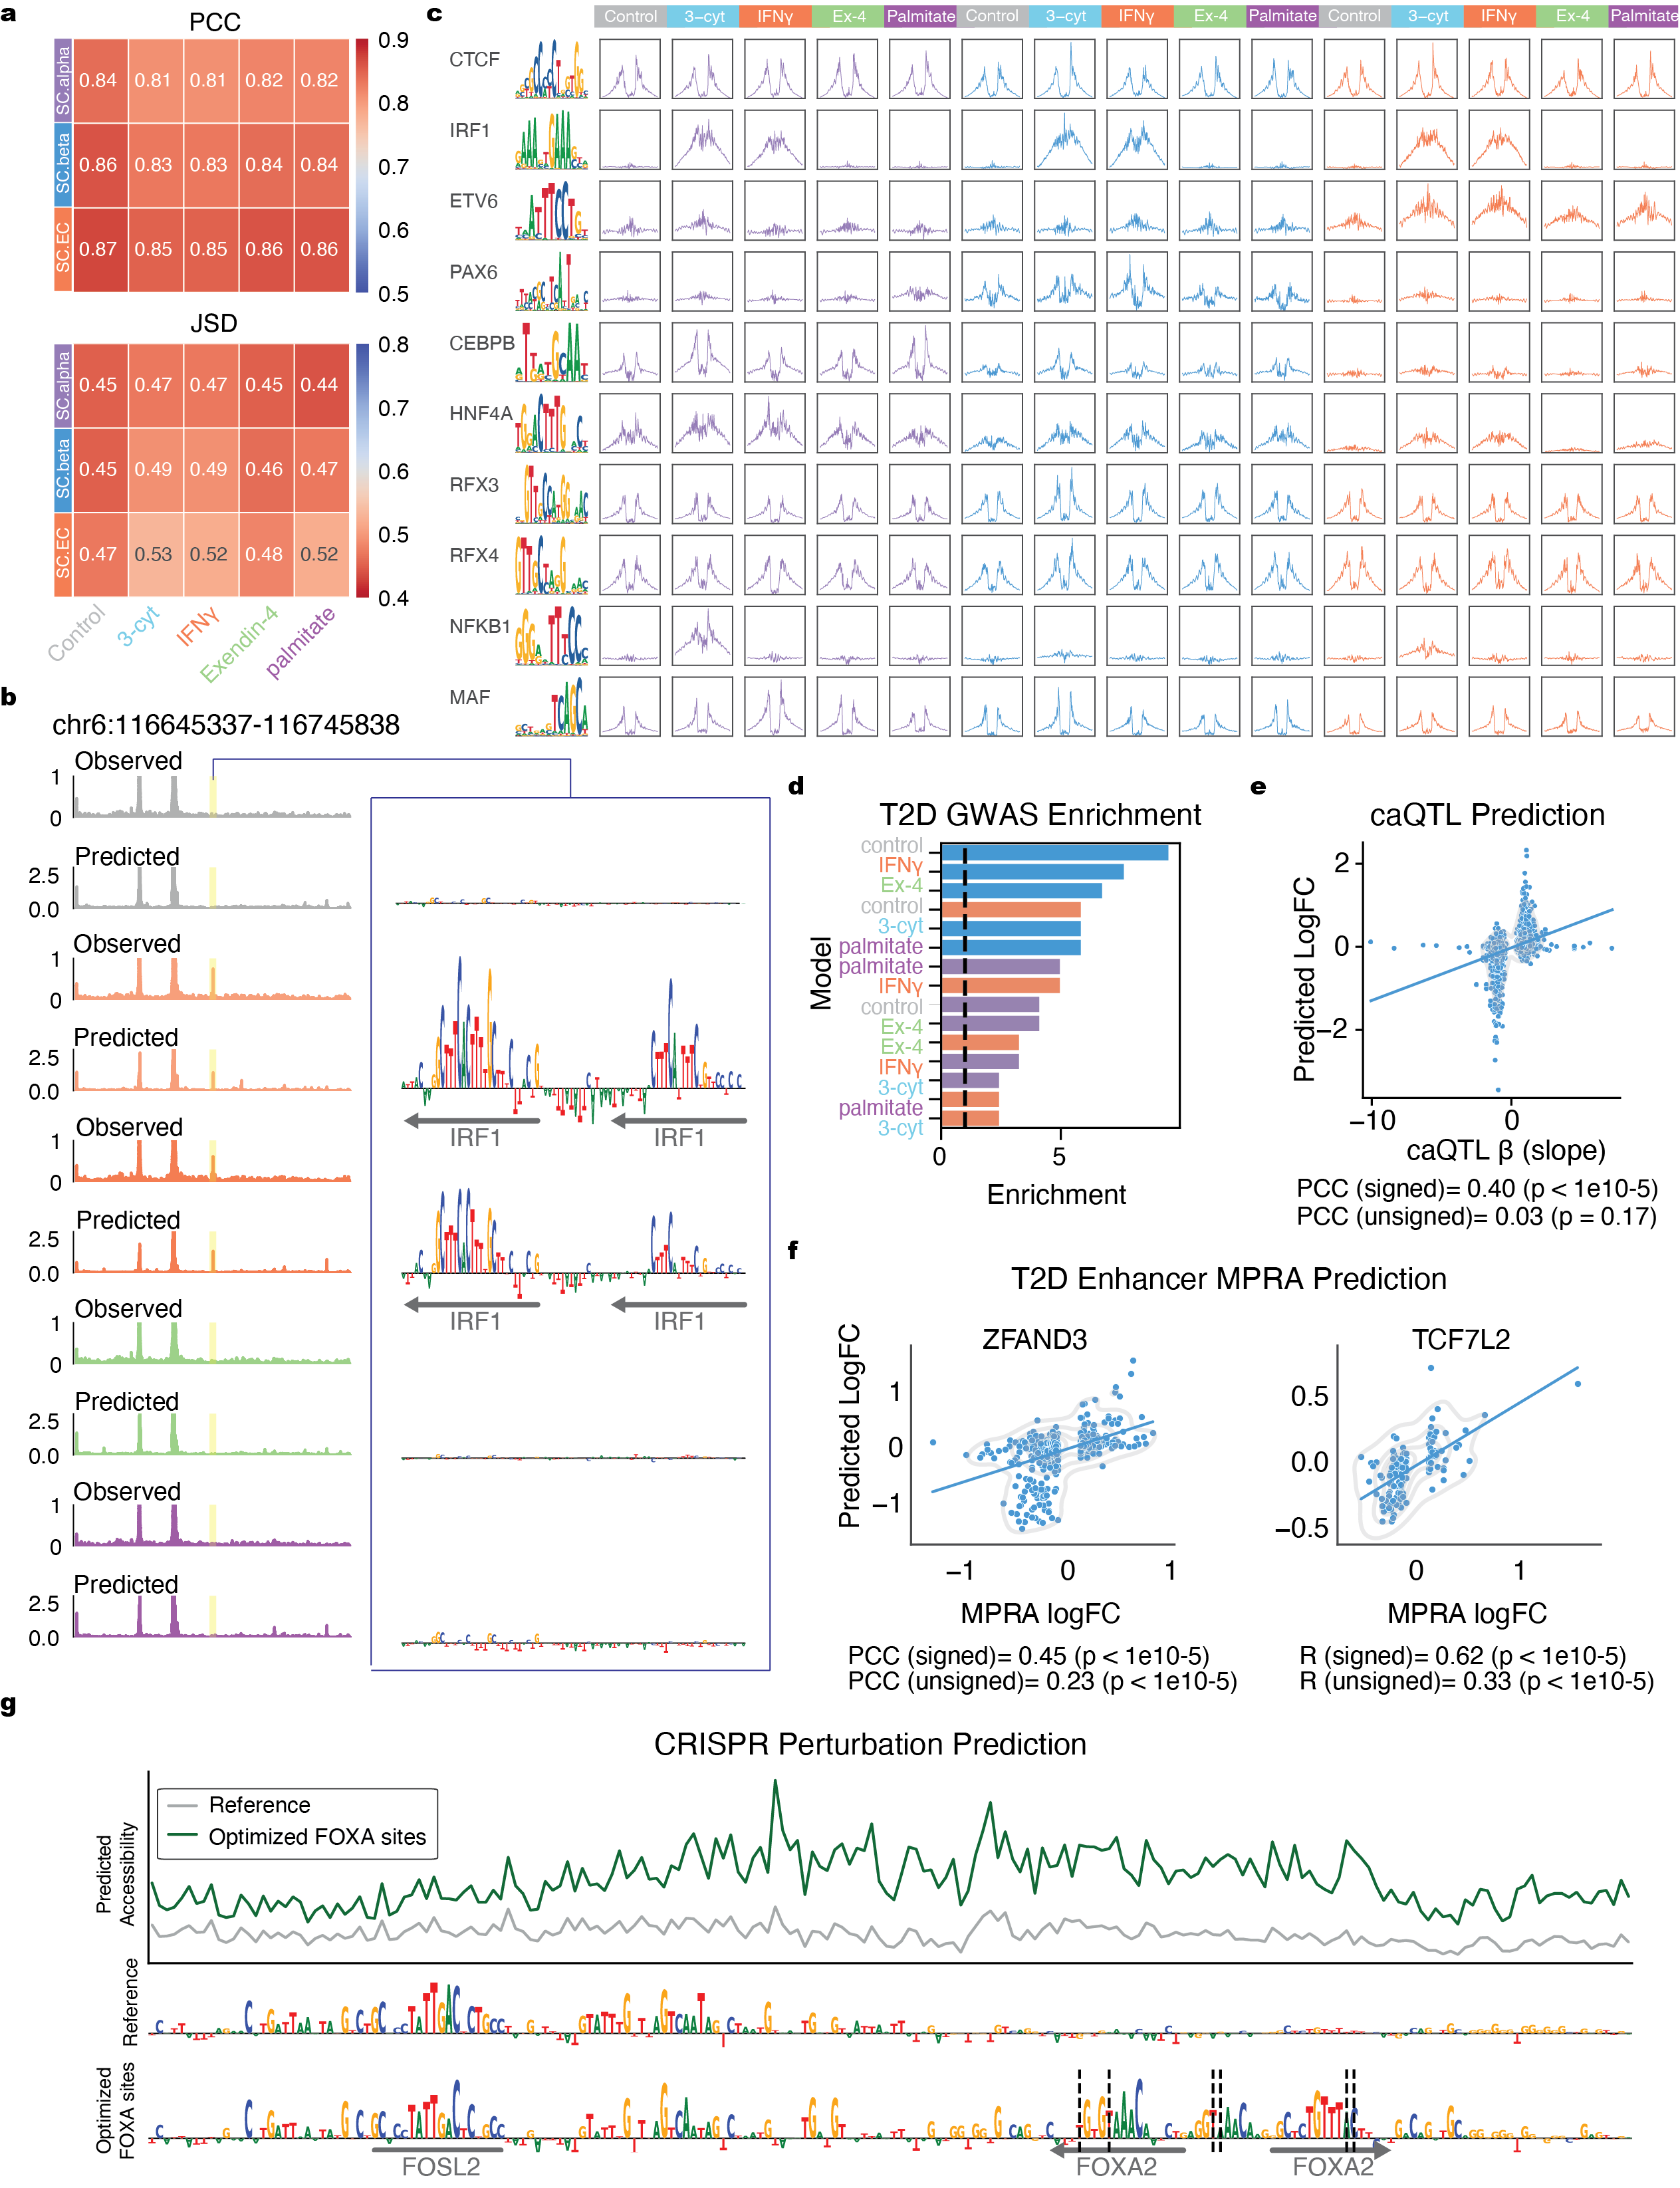
\includegraphics[height=0.8\textheight, keepaspectratio]{3_figures-and-files/Fig4.png}
    \caption[Sequence-to-function models accurately predict condition specific chromatin accessibility and regulatory variant effects]{\textbf{Sequence-to-function models accurately predict condition specific chromatin accessibility and regulatory variant effects}.}
    \label{fig:3 Figure 4}
\end{figure}

\clearpage

%%%%%%%%%%%%%%%%%%%%%%%%%%%%%%%%%%%%%%%%%%%%%%%%%%%%%%%%%%%%%%%%%%%%%%%%%%%%%%%%

\subsection{Predicting DNA methylation levels via sequence models}

We next examined DNA methylation changes in SC-beta cells in response to environmental stimuli. While strong cell type specific differences in methylation at CpGs were observed (\textbf{Figure~\ref{fig:3 Figure 1}\textbf{b}}), condition specific effects within SC-beta cells were comparatively modest (\textbf{Figure~\ref{fig:3 Figure 5}\textbf{a}}). Differential methylation analysis identified fewer than 10 significantly altered regions at a canonical 5\% FDR. By applying a relaxed nominal $p$-value cutoff ($p < 0.0001$), we were able to observe global trends in DNA methylation changes. Specifically, treatment with 3-cyt, IFN$\gamma$, and Exendin-4 was associated with a global decrease in methylation, whereas palmitate exposure induced modest methylation gains across many loci (\textbf{Figure~\ref{fig:3 Figure 5}\textbf{b}}). The subtlety of these observed patterns may reflect a lack of a strong effect of these stimuli on CpG methylation, but it remains possible that the timeframe used in this study is insufficient to capture more extensive DNA methylation changes.

To better understand how sequence determines CpG methylation patterns, we aimed to develop deep learning models that predict DNA methylation profiles from sequence. Unlike prior models of this type, which often predict binary methylation states at individual CpGs or average methylation across regions \cite{Zeng2017-kb}, our approach aims to improve resolution on both fronts. Specifically, we devised a modeling framework in which we predict the parameters of a beta distribution for each CpG site within a 2,114 bp sequence window (see Methods). This approach provides a measure of uncertainty in the prediction at a given site, while also allowing for point estimates of methylation fractions for performance comparisons (\textbf{Figure~\ref{fig:3 Figure 5}\textbf{c}}). While quantitative prediction performance was modest, classification accuracy was strong across SC-alpha, SC-beta, and SC-EC models (\textbf{Figure~\ref{fig:3 Figure 5}\textbf{d}}). These results suggest that cell type specific methylation patterns are at least partially encoded in the underlying DNA sequence.

\clearpage

\thispagestyle{plain}
\noindent
\textbf{Figure~\ref{fig:3 Figure 5}. Sequence-to-function models accurately classify CpG methylation across cell types}. \textbf{a}, Principal component analysis of pseudobulked DNA methylation profiles from SC-beta cells across all treatment conditions and timepoints. \textbf{b}, Volcano plots showing differential DNA methylation in SC-beta cells across treatments (relative to control). From top left to bottom right: 3-cyt, IFNg, Ex-4\_HG, and palmitate. Positive $\Delta$ indicates increased methylation; negative indicates decreased. Colored points indicate sites with nominal p-value < 0.0001, red-increased, blue-decreased. \textbf{f}, Schematic of deep learning model for predicting methylation profiles from sequence (CpGNet). CpGNet predicts parameters of a beta distribution ($\alpha$, $\beta$) for each CpG in a 2,114 bp window. The parameters can be converted to a point estimate of the methylation fraction using the indicated formula. \textbf{g}, Precision–recall curves showing classification performance of methylation models across cell types. Area under the PR curve (auPRC) is reported for each model in parentheses. The gray dashed line represents the performance of a random classifier.

\clearpage

\begin{figure}[!htbp]
    \centering
    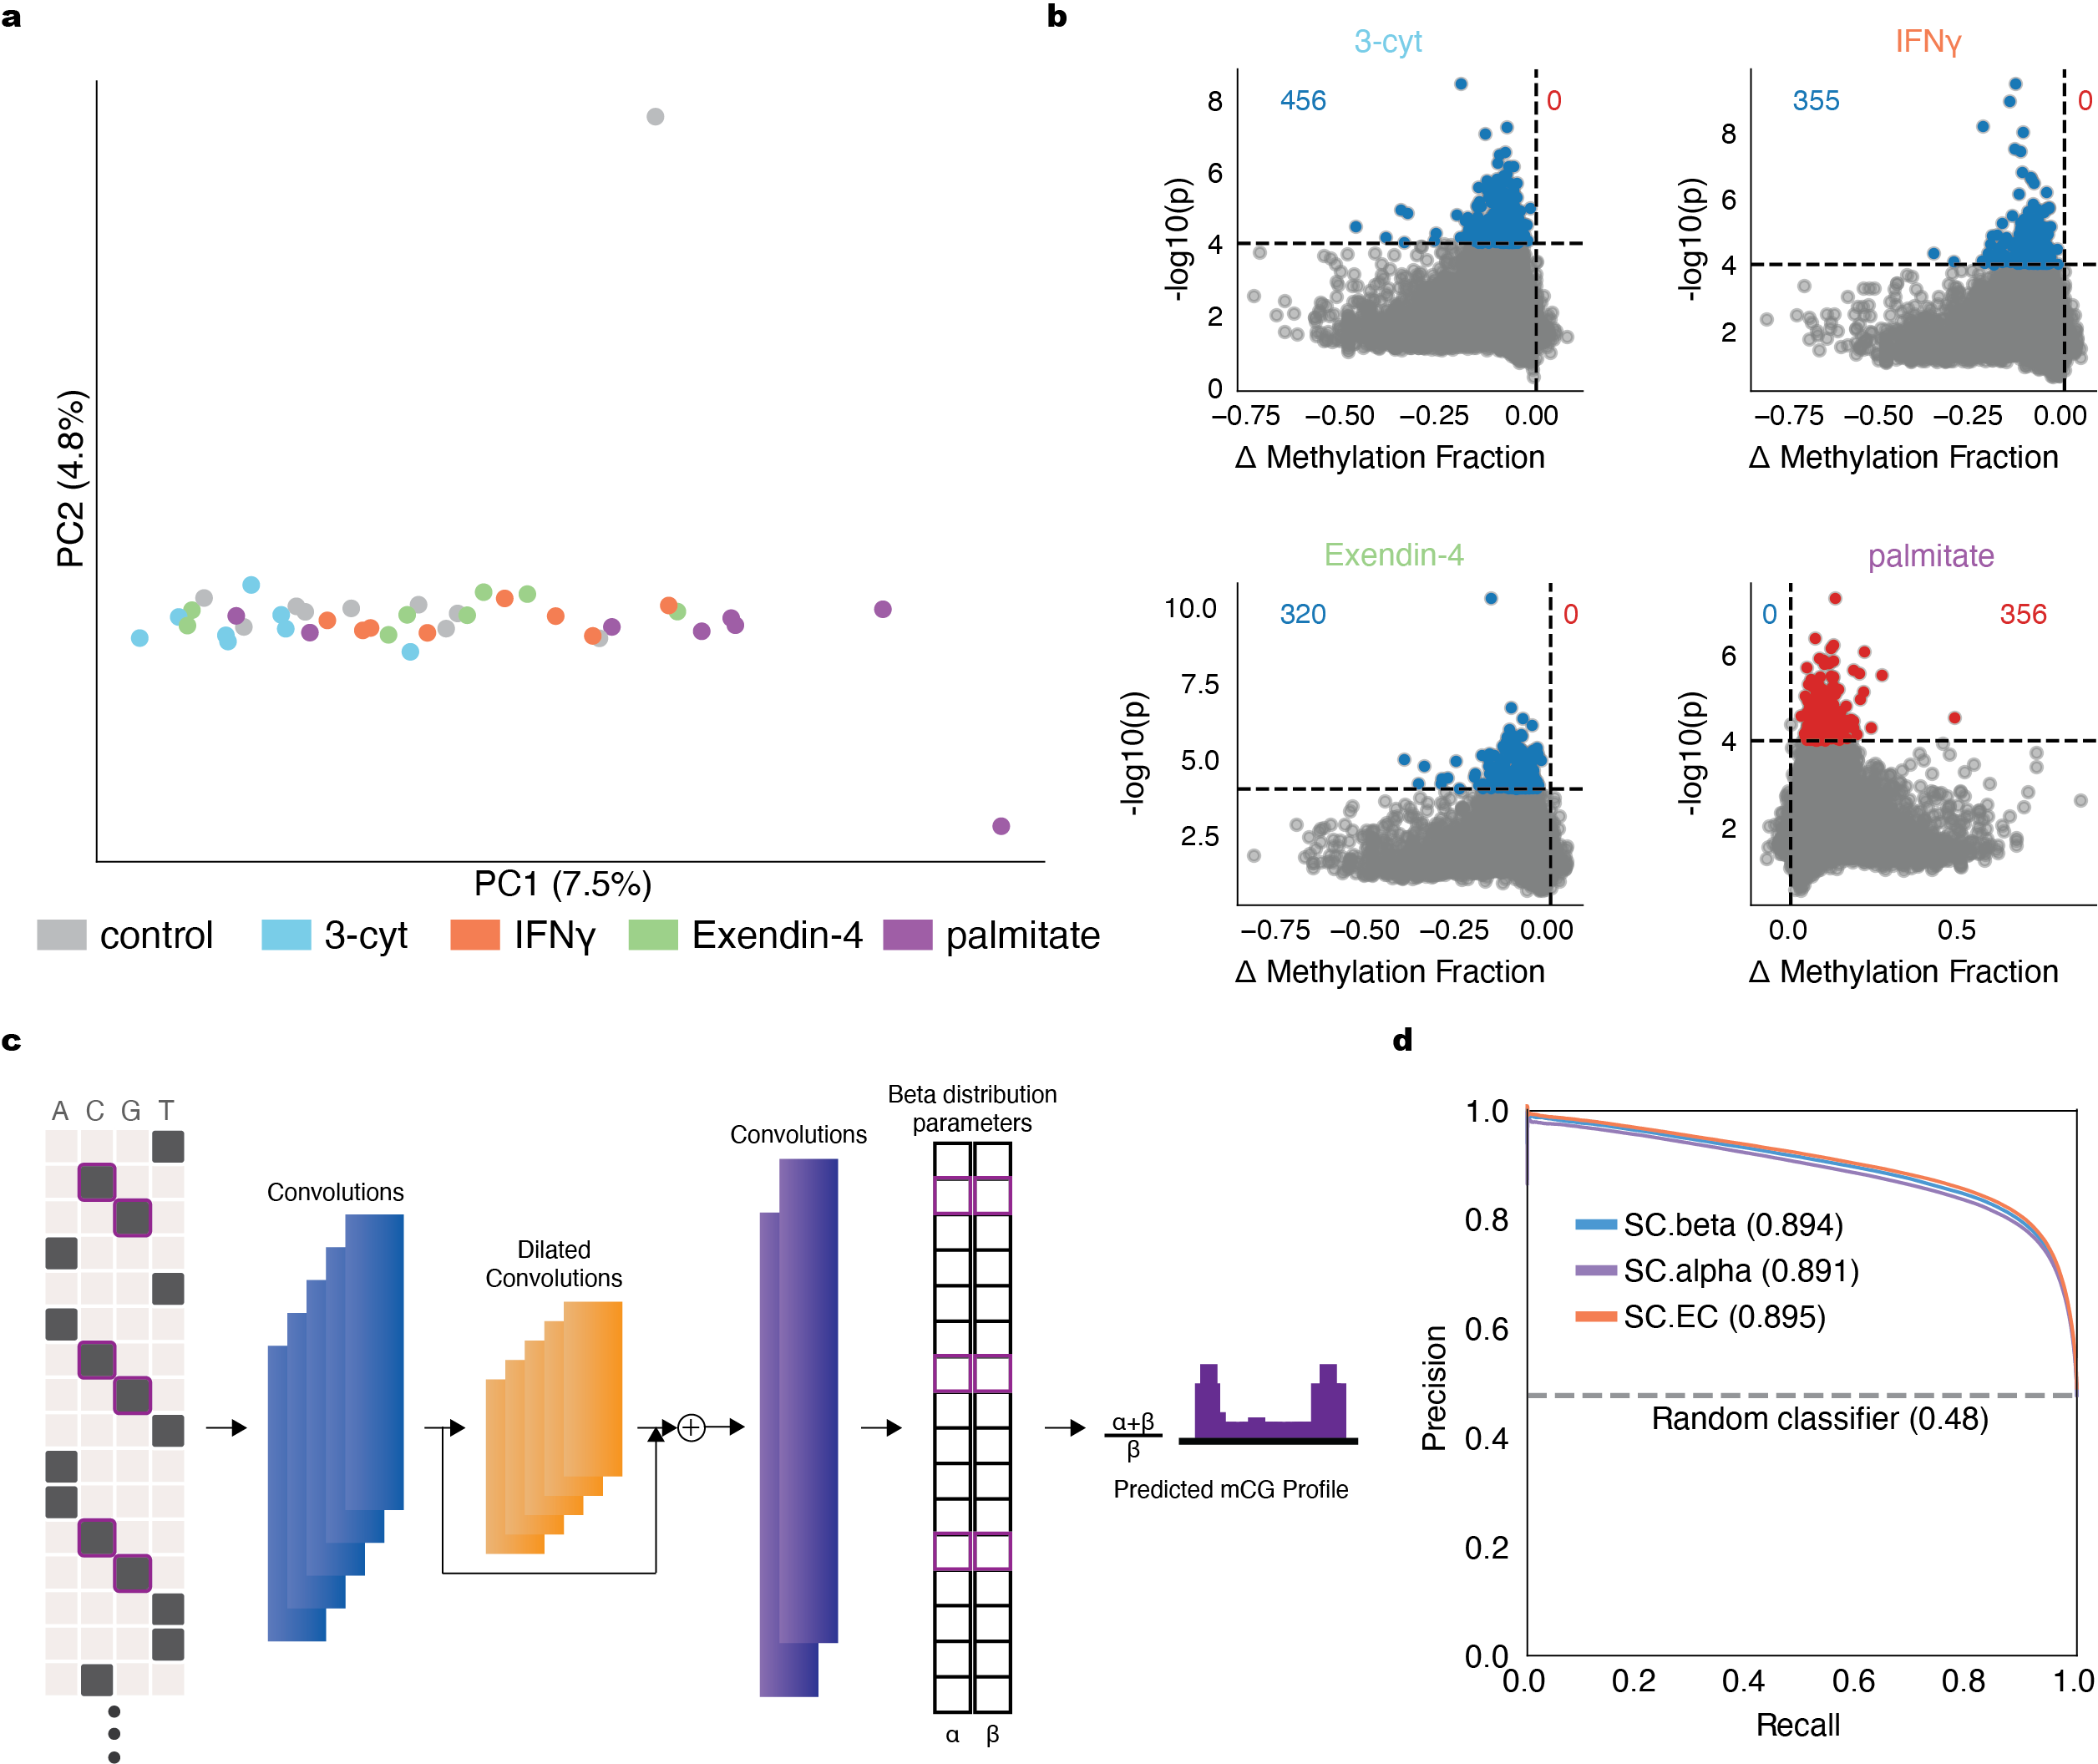
\includegraphics[height=0.65\textheight, keepaspectratio]{3_figures-and-files/Fig5.png}
    \caption[Sequence-to-function models accurately classify CpG methylation across cell types]{\textbf{Sequence-to-function models accurately classify CpG methylation across cell types}.}
    \label{fig:3 Figure 5}
\end{figure}

\clearpage

%%%%%%%%%%%%%%%%%%%%%%%%%%%%%%%%%%%%%%%%%%%%%%%%%%%%%%%%%%%%%%%%%%%%%%%%%%%%%%%%
\section{Discussion}
%%%%%%%%%%%%%%%%%%%%%%%%%%%%%%%%%%%%%%%%%%%%%%%%%%%%%%%%%%%%%%%%%%%%%%%%%%%%%%%%

Our differential analyses revealed condition specific dynamics across gene expression, chromatin accessibility, and DNA methylation, but understanding how these layers interact requires an integrated framework. Work to construct gene regulatory networks (GRNs) by linking transcriptional regulators to the CREs they bind and the CREs to the genes they target \cite{Levine2005-je,Badia-I-Mompel2023-fu} is ongoing. Preliminary CRE-to-gene links derived from our multiome data are enriched for variants from T2D GWAS and other traits related to $\beta$-cell function (not shown here). Together with predictions of TF binding sites from our chromatin accessibility models (not shown), these links form the basis for constructing cis-GRNs for each gene. Importantly, because our data span multiple conditions and timepoints, networks could be used to identify dynamic pathways that are selectively rewired under different stimuli. In our cytokine treatments, for example, we would expect to observe a subnetwork consisting of sharp inflammation-specific TF, enhancer, and downstream effector gene activation involving the canonical regulators STAT1 and IRF1, of important relevance to type 1 diabetes (T1D) \cite{Benaglio2022-rq}. Consolidating these condition-dependent effects into networks will offer an interpretable view of the system that can be used to identify convergent mechanisms of genetic risk \cite{Schnitzler2024-xi} and to propose candidates for perturbation and validation.

In this study, we trained deep learning models to predict CpG methylation fractions at base-pair resolution using DNA sequence alone, achieving strong classification accuracy across cell types. Our CpG modeling framework represents a promising step in improving our understanding of how DNA sequence encodes cell type specific methylation patterns, but is in its early stages and several open questions remain. Future work is needed to evaluate alternative definitions of the training set, key modeling parameters, and model architectures. Loss functions that account for coverage, such as a beta-binomial likelihood–based objective \cite{Dolzhenko2014-mw}, could improve confidence estimation and model fit, especially in low-coverage regions. Interpretation of models also remains a major challenge, as work is needed to determine whether existing attribution methods can generalize to methylation data, and if not, what alternatives should be used. Improved training strategies, model architectures, and interpretation methods will provide an improved lens for identifying genetic variants that alter DNA methylation in a cell type specific manner \cite{Zeng2017-kb}.

Our \textit{in silico} predictions of \textit{NKX6-1} enhancer-optimizing variants closely matched experimental results from CRISPR-Cas9 editing \cite{Geusz2021-mr}, suggesting the potential of such models for the rational design of CREs that enhance gene expression in this system. One particularly compelling application of this approach would be to reduce the proportion of SC-EC cells observed in the differentiation. The molecular profiles of these cells are similar to those observed in fetal $\beta$-cells and arise during differentiation as an alternative fate to SC-beta cells \cite{Zhu2023-qm}. In complementary ongoing work, we have identified several candidate genes that influence this fate decision and putative CREs that regulate these genes. By predicting the sequence edits that increase accessibility of such CREs and then engineering them into hPSCs \cite{Porto2020-ve,Komor2016-px}, we may be able to generate SC-islets that have a higher proportion of cells with genomic profiles that match more closely to mature $\beta$-cells. Our initial results provide evidence that this strategy is feasible, suggesting a way forward for manipulating the differentiation to engineer better model systems with therapeutic potential \cite{Liu2023-kd}.

Ultimately, we aim to construct a single model capable of predicting gene expression from DNA sequence alone. This is typically a more difficult problem that requires very large datasets and models that use a much larger genomic context (i.e., on the Mb scale). However, recent work has shown that fine-tuning models such as Borzoi \cite{Linder2025-or} can lead to strong expression prediction when transferred to individual single-cell datasets \cite{Hingerl2024-qq}. Our dataset offers the unique opportunity to also incorporate chromatin conformation information into the model, which has previously been shown to boost performance \cite{Karbalayghareh2022-gt}. We envision a modeling ecosystem in which both modality specific models and this joint model serve complementary purposes. Models trained on individual modalities (e.g., chromatin accessibility or methylation) that are usually smaller and offer stronger interpretability provide mechanistic insight, while a unified model trained to predict gene expression from all modalities provides stronger functional variant interpretation. Going forward, we foresee a sequence-to-function model framework for predicting transcriptional outcomes across models of $\beta$-cells.

Finally, a key future direction for this work is to directly link our molecular readouts to phenotypic measurements of $\beta$-cell function. While we anticipate our final models will accurately predict chromatin accessibility, DNA methylation, and gene expression, our ultimate goal is to predict how non-coding variants influence $\beta$-cell mediated insulin secretion. We plan to perform glucose-stimulated insulin secretion assays \cite{Velazco-Cruz2019-yq} across our panel of conditions, and aim to use our GRNs and sequence models to prioritize variants that have a direct impact on $\beta$-cell function.

%%%%%%%%%%%%%%%%%%%%%%%%%%%%%%%%%%%%%%%%%%%%%%%%%%%%%%%%%%%%%%%%%%%%%%%%%%%%%%%%
\section{Materials and Methods}
%%%%%%%%%%%%%%%%%%%%%%%%%%%%%%%%%%%%%%%%%%%%%%%%%%%%%%%%%%%%%%%%%%%%%%%%%%%%%%%%

\subsection{Islet organoid differentiation and treatment with stimuli}

\subsubsection{Differentiation protocol}

H1 hESCs (male) were maintained as described by Geusz et al. \cite{Geusz2021-mr}. In brief, hESCs were seeded onto Matrigel (Corning, 356238)–coated tissue culture surfaces in mTeSR1 medium (Stem Cell Technologies, 85850) supplemented with 1\% Penicillin-Streptomycin (Thermo Fisher Scientific, 15140122), and propagated every 3 to 4 days. An Accutase (Thermo Fisher Scientific, 00-4555-56)–based enzymatic dissociation method was employed for passaging, and 10~$\mu$M Y-27632 (Stem Cell Technologies, 72307) was supplied on the first day of each passage.

H1 hESCs were differentiated into SC-islets using a protocol we modified from previous publications by Zhu et al. \cite{Zhu2023-qm}. After dissociation using Accutase, H1 cells were suspended in mTeSR1 medium supplemented with 1\% Penicillin-Streptomycin and 10~$\mu$M Y-27632 and plated in 2D at a concentration of $5.7 \times 10^5$ cells/cm$^2$ in a 37$^{\circ}$C incubator. The following day (day 0), undifferentiated cells were washed with Stage 1/2 base medium (see below) and then differentiated using a seven-step protocol with stage-specific media. On day 29, cells were dissociated with Accutase, suspended in Stage 7 medium supplemented with 10~$\mu$M Y-27632, and reaggregated at a concentration of $3 \times 10^6$ cells/well in a low-attachment 6-well plate on an orbital shaker (100~rpm, $0.2 \times g$) in a 37$^{\circ}$C incubator. The speed of the shaker was increased to 110~rpm ($0.3 \times g$) on the following day. Medium was refreshed daily until day 32.

Base medium for all stage-specific formulations was composed of MCDB 131 medium (Thermo Fisher Scientific, 10372019) supplemented with NaHCO$_3$ (Sigma, S6297), GlutaMAX (Thermo Fisher Scientific, 35050061), D-glucose (Sigma, G8769), and BSA (Lampire Biological Laboratories, 7500804) at the following concentrations:

\begin{itemize}
  \item \textbf{Stage 1/2 base medium:} MCDB 131, 1.5~g/L NaHCO$_3$, 1X GlutaMAX, 10~mM D-glucose, 0.5\% BSA
  \item \textbf{Stage 3/4 base medium:} MCDB 131, 2.5~g/L NaHCO$_3$, 1X GlutaMAX, 10~mM D-glucose, 2\% BSA
  \item \textbf{Stage 5/6 base medium:} MCDB 131, 1.5~g/L NaHCO$_3$, 1X GlutaMAX, 20~mM D-glucose, 2\% BSA
  \item \textbf{Stage 7 base medium:} MCDB 131, 1.5~g/L NaHCO$_3$, 1X GlutaMAX, 2\% BSA
\end{itemize}

Media compositions for each stage were as follows:

\begin{itemize}
  \item \textbf{Stage 1 (days 0–3):} base medium, 100~ng/mL Activin A (R\&D Systems, 338-AC/CF), 25~ng/mL Wnt3a (R\&D Systems, 5036-WN; day 0 only)
  \item \textbf{Stage 2 (days 4–6):} base medium, 0.25~mM L-Ascorbic Acid (Sigma, A4544), 50~ng/mL FGF7 (R\&D Systems, 251-KG)
  \item \textbf{Stage 3 (days 7–8):} base medium, 0.25~mM L-Ascorbic Acid, 50~ng/mL FGF7, 0.25~$\mu$M SANT-1 (Sigma, S4572), 1~$\mu$M Retinoic Acid (Sigma, R2625), 100~nM LDN193189 (Stemgent, 04-0074), 1:200 ITS-X (Thermo Fisher Scientific, 51500056), 200~nM TPB (Calbiochem, 565740)
  \item \textbf{Stage 4 (days 9–11):} base medium, 0.25~mM L-Ascorbic Acid, 2~ng/mL FGF7, 0.25~$\mu$M SANT-1, 0.1~$\mu$M Retinoic Acid, 200~nM LDN193189, 1:200 ITS-X, 100~nM TPB
  \item \textbf{Stage 5 (days 12–14):} base medium, 0.25~$\mu$M SANT-1, 0.05~$\mu$M Retinoic Acid, 100~nM LDN193189, 1~$\mu$M T3 (Sigma, T6397), 10~$\mu$M ALK5i II (Cayman Chemicals, 14794), 10~$\mu$M ZnSO$_4$ (Sigma, Z0251), 10~$\mu$g/mL heparin (Sigma, H3149), 1:200 ITS-X
  \item \textbf{Stage 6 (days 15–21):} base medium, 100~nM LDN193189, 1~$\mu$M T3, 10~$\mu$M ALK5i II, 10~$\mu$M ZnSO$_4$, 100~nM $\gamma$-secretase inhibitor XX (Calbiochem, 565789), 10~$\mu$g/mL heparin, 1:200 ITS-X
  \item \textbf{Stage 7 (from day 22):} base medium, 10~$\mu$M ZnSO$_4$, 10~$\mu$g/mL heparin, 1:1000 Trace Element A (Corning, 89408-312), 1:1000 Trace Element B (Corning, 89422-908), 1:100 MEM Non-Essential Amino Acids (Thermo Fisher Scientific, 11140076)
\end{itemize}

\subsection{Condition time courses}

H1 hESCs were differentiated as described above. To initiate treatments, the indicated stimuli were added to stage 7 medium and replenished daily until sample collection at the indicated timepoints:

\begin{enumerate}
    \item a cocktail of proinflammatory cytokines (10~ng/mL IFN-\ensuremath{\gamma} (Peprotech, 300-02), 0.5~ng/mL IL-1\ensuremath{\beta} (Peprotech, 200-01B), 1~ng/mL TNF-\ensuremath{\alpha} (Peprotech, 300-01A))
    \item IFN\ensuremath{\gamma} alone (50~ng/mL)
    \item 0.01~\ensuremath{\mu}M Exendin-4 (Sigma, E7144) with additional glucose to a final concentration of 16.8~mM
    \item 250.0~\ensuremath{\mu}M palmitate (Sigma, P9767) conjugated to fatty acid-free BSA (Sigma, A4612-1G) at a 6:1 molar ratio in 150~mM sodium chloride.
\end{enumerate}

\subsection{Nuclei preparation}

\subsubsection{Sample collection for Chromium single-cell multiome ATAC and gene expression (10X multiome)}

Organoids were cryopreserved in 1~mL stage 7 medium containing 10\% DMSO in a Mr. Frosty at $-80\,^{\circ}\mathrm{C}$ for up to one week, followed by storage at $-80\,^{\circ}\mathrm{C}$.

\subsubsection{Nuclei preparation for Chromium Single Cell Multiome ATAC + Gene Expression (10x multiome)}

Cryopreserved organoids were thawed, then resuspended in 10~mL of ice-cold PBS and centrifuged for 500~rcf, 5~min at 4~\ensuremath{^{\circ}}C. Pellets were then resuspended in 1~mL of chilled NIM-DP-L buffer (0.25~M sucrose, 25~mM KCl, 5~mM MgCl$_2$, 10~mM Tris-HCl pH~7.5, 1~mM DTT, 1X Protease Inhibitor (Pierce), 1~U/\ensuremath{\mu}L Recombinant RNase inhibitor (Promega, PAN2515), and 0.1\% Triton X-100) then added to an ice-cold 1~mL Wheaton dounce homogenizer. Samples were dounce homogenized with a loose pestle (5--10 strokes) to shear large pieces, followed by a tight pestle (15--25 strokes) until the solution was uniform. Homogenate was filtered through a 30~\ensuremath{\mu}m CellTrics filter (Sysmex, 04-0042-2316) into a LoBind tube (Eppendorf, 22431021) and pelleted (1000~rcf, 10~min at 4~\ensuremath{^{\circ}}C) (Eppendorf, 5920 R). The pellet was resuspended in 1~mL NIM-DP buffer (0.25~M sucrose, 25~mM KCl, 5~mM MgCl$_2$, 10~mM Tris-HCl pH~7.5, 1~mM DTT, 1X Protease Inhibitor, 1~U/\ensuremath{\mu}L Recombinant RNase inhibitor) and pelleted (1000~rcf, 10~min at 4~\ensuremath{^{\circ}}C). The pellet was resuspended in 400~\ensuremath{\mu}L Sort Buffer (1~mM EDTA, 1~U/\ensuremath{\mu}L Recombinant RNase inhibitor, 1X Protease Inhibitor, 1\% fatty acid-free BSA in PBS) with 2~\ensuremath{\mu}M 7-AAD (Invitrogen, A1310). 120{,}000 7-AAD-positive nuclei were sorted (Sony, SH800S) into a LoBind tube containing Collection Buffer (5~U/\ensuremath{\mu}L Recombinant RNase inhibitor, 1X Protease Inhibitor, 5\% fatty acid-free BSA in PBS). Final collection volumes were determined and 5X Permeabilization Buffer (50~mM Tris-HCl pH~7.4, 50~mM NaCl, 15~mM MgCl$_2$, 0.05\% Tween-20, 0.05\% IGEPAL, 0.005\% Digitonin, 5\% fatty acid-free BSA in PBS, 5~mM DTT, 1~U/\ensuremath{\mu}L Recombinant RNase inhibitor, 5X Protease Inhibitor) was added to achieve a 1X solution. Nuclei were incubated on ice for 1 minute, then centrifuged (500~rcf, 5~min at 4~\ensuremath{^{\circ}}C) in a swinging bucket centrifuge. Supernatant was discarded and 650~\ensuremath{\mu}L of Wash Buffer (10~mM Tris-HCl pH~7.4, 10~mM NaCl, 3~mM MgCl$_2$, 0.1\% Tween-20, 1\% fatty acid-free BSA in PBS, 1~mM DTT, 1~U/\ensuremath{\mu}L Recombinant RNase inhibitor, 1X Protease Inhibitor) was added without disturbing the pellet followed by centrifugation (500~rcf, 5~min at 4~\ensuremath{^{\circ}}C) in a swinging bucket centrifuge. Supernatant was removed, and the pellet was resuspended in 7~\ensuremath{\mu}L of 1X Nuclei Buffer (Nuclei Buffer (10x Genomics), 1~mM DTT, 1~U/\ensuremath{\mu}L Recombinant RNase inhibitor). 1~\ensuremath{\mu}L was used for counting on a hemocytometer after staining with Trypan Blue (Invitrogen, T10282). 18{,}000 nuclei were used for tagmentation reaction and 10x Genomics controller loading. Then libraries were generated following the manufacturer’s recommended protocol (\url{https://www.10xgenomics.com/support/single-cell-multiome-atac-plus-gene-expression}). 10x multiome ATAC-seq and RNA-seq libraries were paired-end sequenced on a NextSeq 2000, 550 or Element AVITI to assess data quality. If data quality was satisfactory, libraries were deep sequenced on a NovaSeq 6000 or NovaSeq X Plus to a target depth of \textasciitilde50{,}000 reads per cell for each modality.

\subsubsection{Sample collection for smn3c-seq DNA methylation and chromatin capture analysis}

Organoids were transferred to Eppendorf tubes and centrifuged at 500~rcf, 5~min at 4~\ensuremath{^{\circ}}C. Pellets were then washed with 1~mL of room-temperature PBS and centrifuged at 500~rcf, 5~min at 4~\ensuremath{^{\circ}}C. Pellets were resuspended in room-temperature sterile PBS containing 1\% methanol-free formaldehyde (Sigma, F8775) and incubated on a rotator for 10 minutes at room temperature. Cross-linking reactions were quenched by adding glycine (Thermo Fisher Scientific, J16407.36) to a final concentration of 0.2~M and rotated for 5 minutes at room temperature. Samples were centrifuged at 500~rcf, 5~min at 4~\ensuremath{^{\circ}}C and washed twice with 1~mL ice-cold PBS. Cross-linked pellets were snap-frozen in liquid nitrogen following careful removal of the supernatant.

\subsubsection{Nuclei isolation and Fluorescence Activated Nuclei Sorting (FANS) for snm3C-seq}

Crosslinked organoid pellets were subjected to in situ 3C following the steps in the Arima-3C Single Cell Beta Kit (Arima Genomics), with some modifications. First, pellets were resuspended in 20\ensuremath{\mu}L of lysis buffer (Arima-3C Single Cell Beta Kit (Arima Genomics)) and incubated on ice for 30 minutes. 24\ensuremath{\mu}L of Conditioning Solution was added, then transferred to a 0.2 mL PCR tube, and mixed gently by pipetting. Tubes were incubated at \ensuremath{62^{\circ}}C for 30 min in a thermal cycler, with the lid temperature set to \ensuremath{85^{\circ}}C. 20\ensuremath{\mu}L of Stop Solution 2 was added, and mixed gently by pipetting. Tubes were incubated at \ensuremath{37^{\circ}}C for 15 min in a thermal cycler with a lid temperature set to \ensuremath{85^{\circ}}C. 28\ensuremath{\mu}L of the restriction enzyme digestion mix (9.8\ensuremath{\mu}L water, 9.2\ensuremath{\mu}L Buffer H, 4.5\ensuremath{\mu}L Enzyme H1, 4.5\ensuremath{\mu}L Enzyme H2) was added and gently pipette mixed. Tubes were incubated in a thermal cycler for \ensuremath{37^{\circ}}C for 60 min, \ensuremath{65^{\circ}}C for 20 min, then \ensuremath{25^{\circ}}C for 10 min. 82\ensuremath{\mu}L of ligation mix was added (70\ensuremath{\mu}L Buffer C, 12\ensuremath{\mu}L Enzyme C) and gently mixed by pipetting, then incubated at \ensuremath{25^{\circ}}C for 15 min. Sample was transferred to a tube containing 850\ensuremath{\mu}L 1\% BSA in DPBS on ice and filtered through a 30\ensuremath{\mu}m Celltrics strainer to a new tube on ice. Sample was centrifuged at 1,000 \ensuremath{	imes} g for 10 min at \ensuremath{4^{\circ}}C (in bucket rotor). Supernatant was removed and pellets were resuspended each sample in 800\ensuremath{\mu}L of 1\% BSA in DPBS. Nuclei were stained with DRAQ7 at 1:200 and mixed gently with a pipette and incubated on ice for 5 min. One tube of Proteinase K (Zymo cat. no. D3001-2-D) was dissolved in 1 mL of Proteinase K Resuspension Buffer (Zymo cat. no. D3001-2-B) then added to a mix of 15 mL M-Digestion Buffer 2x (Zymo cat. no. D5021-9) and 14 mL water to make pK Digestion Buffer. 2\ensuremath{\mu}L of pK Digestion Buffer were added to each well of an Eppendorf twin.tec\textsuperscript{\textregistered} PCR Plate 384 LoBind\textsuperscript{\textregistered}, skirted, 45 \ensuremath{\mu}L, PCR clean (Eppendorf cat. No. 0030129547). Single DRAQ7 positive nuclei were sorted into individual wells of the 384-well plate using a Sony SH800 cell sorter. Plates were sealed then incubated in a thermal cycler at \ensuremath{50^{\circ}}C for 20 min with a heated lid at \ensuremath{85^{\circ}}C for nuclei digestion.

\subsubsection{Library preparation and Illumina sequencing for snm3C-seq}

The snm3C-seq samples followed the library preparation protocol detailed previously \cite{Lee2019-qo,Liu2021-km}. This protocol has been automated using the Beckman Coulter Biomek i7 liquid handlers for reactions in 384 and 96-well plates. The snm3C-seq libraries were shallow sequenced on the Illumina NextSeq 2000 or Element AVITI to 2--10M reads to check quality. Successful libraries were deeply sequenced on the NovaSeq 6000 or NovaSeq X Plus instruments, using one lane of 25B flow cell per 4 384-well plates and using 150~bp paired-end mode.

\subsection*{10x multiome sequence data analysis}

\subsubsection{Mapping}
Raw sequencing data were processed using \texttt{cellranger-arc} v2.0.0 (10x Genomics), generating single-nucleus RNA-seq (snRNA-seq) unique molecular identifier (UMI) count matrices for intronic and exonic reads mapping in the sense ($5'$) direction of a gene. CellRanger reference data is available at: \url{https://cf.10xgenomics.com/supp/cell-arc/refdata-cellranger-arc-GRCh38-2020-A-2.0.0.tar.gz}

\subsubsection{Sample level QC}
For snRNA-seq, barcodes were retained if they had between 500--7{,}000 detected genes, $<$3\% mitochondrial reads, and $<$1\% ribosomal reads. Ambient RNA contamination was removed using SoupX \cite{Young2020-qv}, leveraging a curated set of islet-specific marker genes to inform the background model. Doublets were identified using a consensus approach combining Scrublet \cite{Wolock2019-hq}, scDblFinder \cite{Germain2021-uf}, and CellRanger's built-in multiplet detection, with cells removed if flagged by any method. For the ATAC modality, barcodes were retained if they had between 1{,}000--1{,}000{,}000 fragments and a transcription start site enrichment (TSSe) score $\geq 5$. ATAC doublets were identified using AMULET \cite{Thibodeau2021-gy} and Scrublet, and were removed if flagged by either method.

\subsubsection{RNA clustering and cell type annotation}
Expression matrices from all samples were merged, then normalized using total count scaling to a target value of 10{,}000 corrected UMI counts for each cell. Expression values were then log transformed with a pseudocount and the top 3{,}000 variable genes were selected using a dispersion-based approach \cite{Satija2015-rq}. Total UMI counts and percent mitochondrial counts were then regressed out using linear regression. The resulting matrix was scaled and principal component analysis (PCA) was performed to reduce dimensions and noise. Batch correction was performed with Harmony \cite{Korsunsky2019-pn} on PCA embeddings using sample as the correction variable. A $k$-nearest neighbor graph was constructed using $k = 30$ and cell clustering was performed using Leiden (resolution = 1.0). A first round of cell annotation was performed manually using known cell type markers (\textbf{Table S2}). Cell cycle scores were calculated based on a published gene set \cite{Tirosh2016-xd}. Non-endocrine clusters and a proliferating cell cluster were removed upon which the above analysis was repeated.

\subsubsection{ATAC clustering}
We partitioned the hg38 genome into 5-kilobase (kb) sliding windows and removed windows overlapping blacklisted regions from ENCODE (\url{http://mitra.stanford.edu/kundaje/akundaje/release/blacklists/hg38-human/hg38.blacklist.bed.gz}). We generated a barcode-by-window count matrix consisting of the counts of Tn5 insertions within each 5~kb window for each barcode. We selected the 250{,}000 most accessible windows and performed dimensionality reduction via TF-IDF transformation and spectral embedding. The first principal component (PC) was removed from further analysis as it was strongly correlated with read depth. The remaining PCs were corrected with Harmony on sample and a $k$-nearest neighbor graph was constructed using $k = 30$. Cell clustering was performed using Leiden (resolution = 1.0) and clusters which contained $<$100 cells and those that represented possible progenitor-like ATAC states were removed. This analysis was repeated with the remaining barcodes in the same manner with exception to the resolution of Leiden clustering which was increased to 2.5. Again, clusters which contained $<$100 cells were removed.

For all downstream analysis, only the 171{,}815 barcodes present in both the final RNA and ATAC clusters were retained.

\subsubsection{Peak calling and pseudobulking ATAC-seq}
Fragments for each of the four major endocrine cell types (SC-alpha, SC-beta, SC-EC and SC-delta) were combined and cell type specific peak calling was performed using MACS3 \cite{Zhang2008-vm} (via SnapATAC2 v2.5.3 \cite{Zhang2024-kb}) with the following parameters: \texttt{--qval 0.05}, \texttt{--shift -100}, \texttt{--extsize 200}, and \texttt{--min-length 200}. No control or replicate input was used, and the \texttt{--nolambda} setting disabled local background modeling. Consensus peak sets were constructed by expanding peak summits $\pm 250$~bp, merging cell type specific peaks sets (union), and using an iterative algorithm to resolve overlaps. At each step, the most significant remaining peak (lowest $p$-value) was retained, and all overlapping peaks were excluded. This process was repeated until a fixed-width (501~bp), non-overlapping consensus peak set was obtained across cell types.

For the UMAP presented in \textbf{Figure~\ref{fig:3 Figure 1}b}, we generated a consensus peak matrix by counting Tn5 insertions within each peak across all RNA labeled barcodes. We selected the 250{,}000 most accessible peaks and performed dimensionality reduction via TF-IDF transformation and spectral embedding \cite{Zhang2024-kb}. The first PC was removed from further analysis as it was strongly correlated with read depth. The remaining PCs were corrected with Harmony on sample and a $k$-nearest neighbor graph was constructed using $k = 30$ and cell clustering was performed using Leiden (resolution = 1.0). Base resolution ATAC profiles were generated per cell type and normalized to fragments per million for browser visualization.

\subsubsection{Gene activity scoring and RNA-ATAC correlation}
We also generated a cell by gene activity matrix by counting the Tn5 insertions in the region 2{,}000~bp upstream of each gene’s transcription start site (TSS). We then summed counts across sample and cell type to create a sample-cell type by gene matrix. We did the same for summing for SoupX corrected RNA UMI counts and computed Spearman’s $\rho$ for each gene across sample-cell type combinations. We created a null distribution to compare against by shuffling the sample-cell type labels and repeating the correlation calculations across genes.

\subsection{snm3c-seq data analysis}

\subsubsection{Mapping}

The snm3C-seq FASTQ reads were demultiplexed and mapped using YAP (Yet Another Pipeline) software (cemba-data v1.6.9), as previously described \cite{Liu2021-km}. First, FASTQ files were demultiplexed for each cell barcode. Next, two-pass mapping was performed with bismark  (v0.20), using bowtie2 (v2.3). BAM file processing and QC was performed using samtools  (v1.9) and picard (v3.0.0). Chromatin contacts were called and methylome profiles were generated using Allcools (v1.0.23). All reads were mapped to the hg38 reference genome assembly.

\subsubsection{Sample level QC}

A total of 42 384-well plates (16{,}128 single nuclei) were processed and sequenced across the snm3C-seq experiment. We retained nuclei that passed the following two criteria: (1) detection of $\geq$60{,}000 CpG sites genome-wide (at least one read overlaps), and (2) a global mCG percentage between 60--90\%. After applying these filters, 15{,}535 high-quality nuclei were retained for downstream analyses.

\subsubsection{mCG analysis}

\noindent
\textbf{Variably methylated gene identification} \\
We used MethSCAn \cite{Kremer2024-pd} to identify 46{,}360 variably methylated regions (VMRs). We next generated a pseudobulk smoothed methylation profile across all cells and the entire genome, and quantified the average deviation for all CpGs in each VMR for each cell. We repeated the same process to compute the residual over other features, including gene bodies $\pm$2kb. This created the cell by gene matrix that we used for detecting cell type specific differences in methylation at marker genes.

\noindent
\textbf{mCG Clustering and cell type annotation} \\
We used an iterative PCA procedure on the the residual matrix to generate low-dimensional embeddings \cite{Kremer2024-pd}, followed by Leiden clustering (resolution\,=\,0.2). Progenitor-like clusters were identified based on reduced methylation at known progenitor marker genes and removed from further analysis, resulting in a filtered dataset of 14{,}197 cells. The analysis pipeline was then repeated on this subset to identify VMRs, generate residual methylation matrices, and cluster with an increased Leiden resolution of 0.5. Cell types were manually annotated based on methylation patterns at well-characterized marker genes.

\noindent
\textbf{mCG pseudobulking} \\
After mapping, single-cell DNA methylome profiles of the snm3C-seq datasets are stored in the `all cytosine' (ALLC) format, which is a tab-separated table compressed and indexed by bgzip/tabix. For pseudobulk analyses, we averaged methylation fractions across nuclei grouped by sample and cell type. Additionally, we calculated average methylation levels within predefined genomic features, including gene bodies $\pm$2kb, promoters (TSS $\pm$2kb), previously defined VMRs, and consensus ATAC peaks, enabling comparisons across modalities and conditions.

To assess the concordance between methylation and other molecular modalities, we computed Spearman’s rank correlation ($\rho$) between pseudobulk methylation values and the corresponding RNA expression levels for each gene across sample-cell type groups. We also computed analogous correlations between methylation and chromatin accessibility within ATAC peaks. Null distributions were generated by permuting the sample-cell type labels and repeating the correlation analyses across features.

\subsubsection{3D genome analysis}

\noindent
\textbf{Generating the chromatin contact matrix and imputation} \\
After snm3C-seq mapping, we used the cis long-range contacts (contact anchors distance\,$>$\,1{,}000\,bp) and trans contacts to generate single-cell raw chromatin contact matrices at three genome resolutions: chromosome 100\,kb resolution for the chromatin compartment analysis; 25\,kb bin resolution for the chromatin domain boundary analysis; and 10\,kb resolution for the chromatin loop or dot analysis. The raw cell-level contact matrices are stored in HDF5-based scool format. We then used the \texttt{scHiCluster} \cite{Zhou2019-vd} package (v.1.3.2) to perform contact matrix imputation. In brief, the \texttt{scHiCluster} imputes the sparse single-cell matrix in two steps: the first step is Gaussian convolution (pad\,=\,1); the second step is to apply a random walk with restart algorithm on the convoluted matrix. The imputation is performed on each cis matrix (intrachromosomal matrix) of each cell. For 100\,kb matrices, the whole chromosome is imputed; for 25\,kb matrices, we imputed contacts within 10.05\,Mb; for 10\,kb matrices, we imputed contacts within 5.05\,Mb. The imputed matrices for each cell were stored in cool format. For most of the following analyses, cell matrices were aggregated into cell groups identified in the previous section.

\noindent
\textbf{3C gene scores} \\
We computed gene scores using the \texttt{scHiCluster gene-score} command at 10\,kb resolution for both single-cell and sample-cell type psuedobulks. To assess the concordance between 3C and RNA, we computed Spearman’s $\rho$ between pseudobulk normalized gene expression and normalized gene scores. A null distributions was generated by permuting the sample-cell type labels and repeating the correlation analyses across sample-celltype labels for each gene.

\subsection{Differential analysis}

\subsubsection{Differential gene expression}

Differential gene expression was performed on pseudobulked snRNA-seq profiles using DESeq2 \cite{Love2014-rn}. SoupX-corrected UMI counts were aggregated across barcodes for SC-beta cells by sample. Counts were normalized using DESeq2’s variance-stabilizing transformation, then differentiation batch effects were removed using limma \cite{Ritchie2015-ec}. PCA was performed as a qualitative assessment of variance sources. To model dynamic transcriptional responses across conditions and timepoints, we used the following full design formula: \texttt{design = \textasciitilde{} differentiation\_batch + timepoint + condition:timepoint}, webserverhere \texttt{differentiation\_batch} represents one of 2 differentiation batches organoids were derived from in this study, \texttt{timepoint} is a factor with levels ``0'', ``6'', ``24'', ``48'', ``72'' and reference value ``0'', and \texttt{condition} was a factor with reference value ``control''. A likelihood ratio test (LRT) was used to compare this full model to a reduced model excluding the interaction term: \texttt{reduced = \textasciitilde{} differentiation\_batch + timepoint}

Formally, the LRT evaluates whether the addition of the \texttt{condition:timepoint} term explains significantly increases the model likelihood compared to the reduced model. Practically, genes with small p-values from this test are those that show a condition specific expression response at one or more timepoints after baseline (\(t = 0\)). P-values were corrected with the DESeq2 default Benjamini-Hochberg method \cite{Benjamini1995-da}.

We next fed the results of the DESeq2 analysis to DecoupleR-py \cite{Badia-I-Mompel2022-se} for TF activity inference analysis. Specifically, we used univariate linear model regression of the estimated log2FC from DESeq2 to infer TF activity weights using the CollecTRI \cite{Muller-Dott2023-zc} network. We define the activity score of a TF as the t-value of the slope coefficient of the regression with a p-value obtained by evaluating the two-sided survival function of the Student’s t-distribution.

Differentially expressed genes (DEGs) were defined as genes with adjusted p-value $<$ 0.05 for cytokines and $<$ 0.25 for Exendin-4 and palmitate and absolute log2FC $>$ 0.5. We then clustered DEGs using \texttt{degPatterns} from the DEGreport package (v1.42.0) with default parameters. Briefly, for each condition and timepoint, gene expression was averaged across samples. Pairwise gene–gene similarity was computed using Kendall correlation, and the resulting distance matrix was clustered using divisive hierarchical clustering (\texttt{cluster::diana}). The number of clusters was determined by the divisive coefficient. Only clusters containing more than 15 genes were retained. For visualization, expression values were scaled using \texttt{scale()}, yielding z-scores per gene.

To functionally annotate clusters, we ran the \texttt{gseapy} \cite{Fang2023-st} implementation of EnrichR \cite{Xie2021-me} against the following gene sets: \texttt{"GO\_Biological\_Process\_2025"}, \texttt{"GO\_Cellular\_Component\_2025"}, \texttt{"GO\_Molecular\_Function\_2025"}, \texttt{"MSigDB\_Hallmark\_2020"}, \texttt{"Reactome\_Pathways\_2024"}, \texttt{"KEGG\_2021\_Human"}. We identified gene clusters with at least one FDR corrected (0.05) hit and visually inspected the heatmap and hits to select the clusters to present in \textbf{Figure~\ref{fig:3 Figure 2}d}.

\subsubsection{Differential chromatin accessibility}

Differential chromatin accessibility was performed on pseudobulked snATAC-seq profiles using DESeq2 \cite{Love2014-rn}. Tn5-corrected insertion counts were aggregated across barcodes for SC-beta cells by sample using the shared consensus peak set (see Methods). Counts were normalized using DESeq2’s variance-stabilizing transformation, then differentiation batch effects were removed using limma \cite{Ritchie2015-ec}. PCA was performed as a qualitative assessment of variance sources. To model dynamic chromatin accessibility responses across conditions and timepoints, we used the following full design formula: \texttt{design = \textasciitilde{} differentiation\_batch + timepoint + condition:timepoint}, where \texttt{differentiation\_batch} represents one of two differentiation batches organoids were derived from, \texttt{timepoint} is a factor with levels ``0'', ``6'', ``24'', ``48'', ``72'' and reference value ``0'', and \texttt{condition} was a factor with reference value ``control''. A likelihood ratio test (LRT) was used to compare this full model to a reduced model excluding the interaction term: \texttt{reduced = \textasciitilde{} differentiation\_batch + timepoint}

Formally, the LRT evaluates whether the addition of the \texttt{condition:timepoint} term significantly increases model likelihood compared to the reduced model. Practically, peaks with small p-values from this test are those that show a condition specific accessibility response at one or more timepoints after baseline (\(t = 0\)). P-values were corrected with the DESeq2 default Benjamini-Hochberg method \cite{Benjamini1995-da}.

Differentially accessible regions (DARs) were defined as peaks with adjusted p-value $<$ 0.05 for cytokines and $<$ 0.25 for Exendin-4 and palmitate. We then clustered DARs using \texttt{degPatterns} in the same manner as DEGs.

To functionally annotate clusters of DARs, we ran motif enrichment using HOMER \cite{Heinz2010-yo}. Each cluster of peaks was analyzed using the \texttt{findMotifsGenome.pl} tool with default settings using the rest of the DARs as background. Clusters with at least one motif passing the default enrichment threshold (adjusted p-value $<$ 0.05) were further examined. We visually inspected the cluster heatmaps and enrichment results to identify representative clusters presented in \textbf{Figure~\ref{fig:3 Figure 3}d}. We also used HOMER’s peak annotation utility to assign each peak to its nearest gene and classify it by genomic context (e.g., promoter, intron, intergenic).

\subsubsection{Differential methylation}

We performed DMR calling as described in MethSCAn \cite{Kremer2024-pd}. Briefly, we slid a 2\,kb window across the genome with a step size of 1\,kb and computed a t-test of average methylation fraction across groups for each window. Windows with a t-statistic in the top 2\% or bottom 2\% were merged if overlapping and reported as DMRs. A minimum of six cells was required per group for a region to be considered for a t-test.

\subsection*{Base-pair resolution chromatin accessibility modeling}

We trained base-pair resolution chromatin accessibility models for each cell type across all the samples from the same condition time course. We therefore had a total of 15 models, one for each cell type (3) and condition (5) combination (including control). We aggregated fragments genome-wide for each cell type and condition for training models. We used peak calls for the cell type across all samples, and subset the peaks to the top 250,000 by q-value for training models.

\subsubsection*{Bias model training}

For bias model training, we used fragments and peaks from the SC-beta control cells. We selected a GC matched set of negative regions \(\sim2\times\) as large as the peak set and trained a bias model according to the ChromBPNet repository \cite{Pampari2025-lm} to predict the raw Tn5 insertion counts in these negative regions. We used a beta value 1.0, as we found that smaller beta values led to bias models that learned an AT bias. Loci were split by chromosome into validation (chr8, chr20), test (chr1, chr3, chr6) and training (rest). Negatives in training chromosomes were used to update model parameters, negatives in validation chromosomes for early stopping, and negatives in the test set for final model evaluation. We ensured that the bias model did not learn TF motifs and instead learned the Tn5 motifs as described in the ChromBPNet repository. We hereafter refer to this model as the ‘bias model’.

\subsubsection*{ChromBPNet model training}

We trained ChromBPNet models for all 15 cell type-treatment combinations as described in the ChromBPNet repository. The same bias model was used for all cell type treatment combinations and we used the same chromosomal splits as in bias model training. We evaluated bias correction and model performance as described in the ChromBPNet repository.

\subsubsection*{Model interpretation}

We used DeepLiftShap \cite{Shrikumar2017-og} to generate base-resolution contribution scores for each nucleotide across all 250,000 cell type specific peaks for each respective model. We computed contribution scores for both the counts head and profile head of all models as described in the ChromBPNet repository. We generated prediction and contribution bigwig tracks for all peaks for each model as described in the ChromBPNet repository.

\subsubsection*{Motif analysis}

\paragraph{Motif discovery and clustering}

For each model, we passed both counts and profile contributions across all peaks to the TF-MoDISco \cite{Shrikumar2018-sb} algorithm via the modisco-lite package (v2.2.1). We used the following parameters for all models: \texttt{n\_seqlets=100000}, \texttt{leiden\_res=2}, \texttt{window=400}, with the rest set to defaults. This step outputs a set of contribution weight matrices (CWMs) representing the discovered motifs for each model and task. We combined all motif CWMs into a single meme file and ran \texttt{gimmemotif} \cite{van-Heeringen2011-tx} \texttt{cluster} on them with a threshold of 0.999 and all other parameters set to defaults. We then ran TomTom \cite{Gupta2007-zw} on each motif using a published database of motifs \cite{Vierstra2020-te}.

\paragraph{Motif marginalization}

For each model and motif, we randomly sampled 100 peaks from the peak set of the corresponding cell type without replacement. We then extracted the genomic sequence corresponding to each peak and dinucleotide shuffled it to create a background set of sequences to marginalize motifs on. We then inserted the consensus for the CWM of each motif into the center of all 100 background sequences and measured the difference in both counts and profile predictions to the background set without the motif. We averaged the difference in counts predictions across all 100 sequences for each model to compute an effect size of that motif on that model. We then two separate ANOVAs for each motif for the effect size distribution across all models using cell type and condition respectively. We corrected for multiple tests with Benjamini-Hochberg \cite{Benjamini1995-da} and manually inspected the top hits. We manually selected ten with visually attributable differences to plot in \textbf{Figure~\ref{fig:3 Figure 4}c}.

\subsubsection{Variant effect prediction}

All variant effect prediction was done using the \texttt{variant-scorer} repository \url{https://github.com/kundajelab/variant-scorer}. Briefly, we used trained ChromBPNet models to predict the effects of single nucleotide substitutions (no indels) on chromatin accessibility. Following the repository, we computed three main metrics for each variant:

\begin{itemize}
    \item \textbf{Change in total accessibility (logFC)}: log fold-change between predicted counts for the alternate and reference alleles:
    \item \textbf{Change in profile shape (signed JSD)}: Jensen-Shannon divergence between predicted profiles, multiplied by the sign of logFC:
    \item \textbf{Integrative effect size (IES)}: Combined effect size from both total coverage and shape:\
\end{itemize}

For each variant set (e.g. T2D credible set with background), we compute effect scores for all variants by first averaging predictions for the forward and reverse strands. To assess the statistical significance of predicted variant effects, we then create an empirical null distribution of variant scores by predicting effects using dinucleotide shuffled versions of reference and alternate sequences. When the number of variants in a variant set was \(> 100{,}000\), we randomly sampled 100{,}000 variants to create the null distribution. Otherwise we performed 10 dinucleotide shuffles per variant. Each variant’s IES was then compared against the null distribution to derive empirical p-values.

\subsubsection{T2D GWAS analysis}

To evaluate all models’ variant effect predictions, we first tested for enrichment of high-scoring variants among fine-mapped type 2 diabetes (T2D) risk loci \cite{Mahajan2022-hu}. We obtained a fine-mapped credible set of T2D-associated variants and used the posterior inclusion probability (PIP) scores to identify likely causal variants. For the analysis presented in \textbf{Figure~\ref{fig:3 Figure 4}d}, we used a PIP threshold of 0.8 to define fine-mapped variants and compared them to the top 1\% of model predictions ranked by IES p-values.

To define a suitable background set, we downloaded common non-coding SNPs (minor allele frequency \(\geq 0.01\)) from dbSNP build 153 \cite{Sherry2001-pk}, and filtered out variants likely to have regulatory function using TURF model scores from RegulomeDB \cite{Dong2023-fh}. We retained only variants with a TURF score $<$ 0.05, resulting in a background set of 581,580 non-coding SNPs. All variants were annotated with reference and alternate alleles from dbSNP.

We predicted variant effects for both the fine-mapped and background SNPs and calculated the empirical enrichment of fine-mapped T2D variants among the top-scoring predictions \cite{Pampari2025-lm}. The observed overlap was compared to the expected overlap under the null hypothesis that high PIP variants (>0.8) are no more likely to be regulatory than low PIP ($<$0.8) and background variants.

\subsubsection{caQTL prediction}

To test if our SC-beta control model predictions align to known variant associations with chromatin accessibility, we used chromatin accessibility quantitative trait loci (caQTLs) from $\beta$-cells in human primary islets \cite{Mummey2024-kx}. We selected a set of SNPs as significant caQTLs ($<$0.05 adjusted p-value) located within \(\pm250\) bp of the center of the corresponding peak it was tested against. This resulted in 2,811 SNPs for the $\beta$-cell caQTL benchmark, for which we computed both signed and unsigned Spearman's (\(\rho\)) between predicted log2FCs and caQTL regression coefficients (betas).

\subsubsection{MPRA prediction}

To assess the SC-beta control model’s ability to predict the regulatory effects of sequence variants, we evaluated its performance on an MPRA dataset from \cite{Kircher2019-di}. This study measured the transcriptional effects of single nucleotide variants (SNVs) using a reporter assay in the MIN6 murine pancreatic $beta$-cell line \cite{Miyazaki1990-zz}. The dataset includes quantitative \(\log_2\) fold-change (FC) measurements of reporter activity for SNVs introduced into two known T2D loci (\textit{TCF7L2} and \textit{ZFAND3}). We computed signed and unsigned Spearman's (\(\rho\)) between predicted log2FC and experimentally measured reporter activity across SNVs within each tested region.

\subsubsection{Optimized NKX6-1 enhancer prediction}

Finally, we used our SC-beta control model to predict the effect of a genome editing experiment that optimized a \textit{NKX6-1} enhancer sequence in SC-islets \cite{Geusz2021-mr}. We extracted the reference and optimized enhancer sequences centered on the edited region and predicted accessibility. We visualized predicted accessibility for both alleles alongside DeepLiftShap contributions and annotated contributing motifs with the \texttt{tangermeme} package (v0.4.0).

\subsection{Base-pair resolution CpG fraction modeling}

We trained cell type specific models to predict CpG methylation fraction at base-pair resolution from DNA sequence alone. To do so, we adapted the BPNet architecture \cite{Avsec2021-sw} to predict the methylation fraction of each CpG site within a 1,000 bp output window from 2,114 bp of input DNA sequence. Dataset construction, model training, and evaluation were all performed with EUGENe \cite{Klie2023-yr}. We call this framework CpGNet.

\subsubsection{Training data}

We first defined training regions by selecting the top 250,000 peaks from our chromatin accessibility data. Each region was extended symmetrically to 2,114 bp by adding 1,057 bp on either side of the summit. We filtered out regions that (1) contained fewer than 25 covered CpG sites, (2) had less than 20\% of CpGs covered, or (3) had more than 0.1\% ambiguous bases (Ns) in the reference genome. For each retained region, we computed CpG coverage and methylation fraction at every CpG site in each cell type separately, treating the data as unstranded. We used the same splits to partition regions into training, validation, and test sets as with chromatin accessibility model training.

\subsubsection{Model architecture and training}

CpGNet accepts a one-hot encoded 2,114 bp input sequence and passes it through a wide convolution (21 bp) with 64 filters to learn motif PWMs. This is followed by four dilated residual convolutional layers with exponentially increasing dilation rates. A final wide convolutional layer predicts two channels across a 1,000 bp target window. These values are passed through a softplus activation to ensure positivity and can be interpreted as the \(\alpha\) and \(\beta\) parameters of a beta distribution when paired with the beta loss function we use for training. Non-CpG sites and CpG sites with fewer than 3 reads of coverage were masked from the loss function during training. The model was optimized using the Adam optimizer \cite{Kingma2014-kn} with a learning rate of 0.0001 and batch size of 128. We fit the model for a maximum of 100 epochs, selecting the model with the best validation loss for test set evaluation.

\subsubsection{Evaluation}

We computed the model's predicted \(\alpha / (\alpha + \beta)\) values at all CpGs with greater than 3 reads of coverage in the test set and compared to the observed methylation fraction at these sites in two ways. First, we treated the observed fractions as a continuous value and compared it to predicted methylation fractions using the Pearson correlation coefficient (PCC). We averaged this across all CpGs and test loci as a global metric of model performance. Second, we binarized observed methylation fractions in the test set using a 0.5 threshold (\(\geq 0.5 =\) methylated) and computed the area under the receiver operating characteristic curve (AUROC) and area under the precision-recall curve (AUPRC).

\subsection{Statistical methods}

TomTom reports significance of alignments of query motifs to a database using the methods described in \cite{Gupta2007-zw}. We used the q-value reported by the webserver tool (\url{https://meme-suite.org/meme/tools/tomtom}) and considered hits to be those alignments with a q-value \(\leq 0.05\) as significant.

%%%%%%%%%%%%%%%%%%%%%%%%%%%%%%%%%%%%%%%%%%%%%%%%%%%%%%%%%%%%%%%%%%%%%%%%%%%%%%%%
\section{Data availability}
%%%%%%%%%%%%%%%%%%%%%%%%%%%%%%%%%%%%%%%%%%%%%%%%%%%%%%%%%%%%%%%%%%%%%%%%%%%%%%%%

All data supporting the findings of this study are available at \url{https://data.igvf.org/}. Background variants used for the GWAS analysis were downloaded from \url{https://www.encodeproject.org/files/ENCFF250UJY/}. GWAS T2D data were downloaded from \url{https://t2d.hugeamp.org/dinspector.html?dataset=Mahajan2022_T2D_Mixed} \cite{Mahajan2022-hu}. caQTL data were obtained in direct correspondence with H.M.M \cite{Mummey2024-kx}. MPRA data for TCF7L2 and ZFAND3 were downloaded from \url{https://kircherlab.bihealth.org/satMutMPRA/} \cite{Kircher2019-di}.

%%%%%%%%%%%%%%%%%%%%%%%%%%%%%%%%%%%%%%%%%%%%%%%%%%%%%%%%%%%%%%%%%%%%%%%%%%%%%%%%
\section{Code availability}
%%%%%%%%%%%%%%%%%%%%%%%%%%%%%%%%%%%%%%%%%%%%%%%%%%%%%%%%%%%%%%%%%%%%%%%%%%%%%%%%

The pipelines used for processing the 10x multiome and snm3c-seq data generated in this work can be found at \url{https://github.com/IGVF-UCSD/igvf_sc-islet_10X-Multiome} and \url{https://github.com/IGVF-UCSD/igvf_sc-islet_snm3c/tree/main}, respectively. Code used for integrative analysis and to reproduce figures can be found at \url{https://github.com/adamklie/ChromBetaNet}. Code used for CpGNet model training and evaluation can be found at \url{https://github.com/adamklie/cpgnet}.

%%%%%%%%%%%%%%%%%%%%%%%%%%%%%%%%%%%%%%%%%%%%%%%%%%%%%%%%%%%%%%%%%%%%%%%%%%%%%%%%
\section{Acknowledgements}
%%%%%%%%%%%%%%%%%%%%%%%%%%%%%%%%%%%%%%%%%%%%%%%%%%%%%%%%%%%%%%%%%%%%%%%%%%%%%%%%

We thank all of members of the Carter, Gaulton, Sander, and Ren labs for their input. This work was supported by the National Institutes of Health [grant number 1U01HG012059]; infrastructure was funded by the National Institutes of Health [grant number 2P41GM103504-11]. H.C. is supported by the Canadian Institute for Advanced Research [award number FL-000655].

%%%%%%%%%%%%%%%%%%%%%%%%%%%%%%%%%%%%%%%%%%%%%%%%%%%%%%%%%%%%%%%%%%%%%%%%%%%%%%%%
\section{Author Contributions Statement}
%%%%%%%%%%%%%%%%%%%%%%%%%%%%%%%%%%%%%%%%%%%%%%%%%%%%%%%%%%%%%%%%%%%%%%%%%%%%%%%%

Study supervision: H.C., K.J.G., M.S., and B.R. Contribution to data generation: M.O., N.R.Z., W.M.B. Contribution to data analysis: A.K., H.Z., M.O., H.M.M., S.L., P.B., G.W., K.Z. Contribution to data interpretation: A.K., H.Z., M.O., H.M.M., S.L., H.C., K.J.G., M.S., and B.R. Contribution to writing the manuscript: A.K., H.Z., M.O., N.R.Z.

%%%%%%%%%%%%%%%%%%%%%%%%%%%%%%%%%%%%%%%%%%%%%%%%%%%%%%%%%%%%%%%%%%%%%%%%%%%%%%%%
\section{Competing Interests Statement}
%%%%%%%%%%%%%%%%%%%%%%%%%%%%%%%%%%%%%%%%%%%%%%%%%%%%%%%%%%%%%%%%%%%%%%%%%%%%%%%%

The authors declare no competing interests.

%%%%%%%%%%%%%%%%%%%%%%%%%%%%%%%%%%%%%%%%%%%%%%%%%%%%%%%%%%%%%%%%%%%%%%%%%%%%%%%%
\section{Inclusion and Ethics Statement}
%%%%%%%%%%%%%%%%%%%%%%%%%%%%%%%%%%%%%%%%%%%%%%%%%%%%%%%%%%%%%%%%%%%%%%%%%%%%%%%%

All research was conducted and is relevant locally.
